\documentclass{thesis}%
\usepackage[T1]{fontenc}%
\usepackage[utf8]{inputenc}%
\usepackage{lmodern}%
\usepackage{textcomp}%
\usepackage{lastpage}%
\usepackage{graphicx}%
\usepackage{caption}%
\usepackage{indentfirst}%
\usepackage{titlesec}%
\usepackage{amsfonts}%
\usepackage{amsmath}%
\usepackage{subfigure}%
\usepackage[none]{hyphenat}%žádné dělení slov
\usepackage{genealogytree}



\DeclareMathOperator*{\argmax}{argmax}

 
\renewcommand{\listfigurename}{Seznam obrázků}
\captionsetup[table]{name=Tabulka}
\captionsetup[figure]{name=Obr.}
\renewcommand\listtablename{Seznam tabulek}
\renewcommand{\contentsname}{Obsah}
\renewcommand{\refname}{Seznam zdrojů}
\renewcommand{\abstractname}{Abstrakt}




\begin{document}%
%TITLE PAGE SETTINGS%
\sloppy %dodržování zarovnání na konce řádky
\begin{titlepage}
    \begin{center}
        \vspace*{0.6cm}
        

        
        \includegraphics[width=0.7\textwidth]{zcu.png}
        
        Západočeská univerzita v Plzni\\
        Fakulta aplikovaných věd\\       
        Katedra kybernetiky\\

        \vspace{4 cm}
     \textbf{DIPLOMOVÁ PRÁCE}
        
        \vspace{0.5cm}
       Modelování cévního řečiště jater s využitím kombinace snímků z trojrozměrných lékařských zobrazovacích metod
        
        \vspace{6cm}
   \end{center}    

\begin{tabular}[t]{@{}l} 
 \textbf{PLZEŇ, 2019}
\end{tabular}
\hfill% move it to the right
\begin{tabular}[t]{l@{}}
   \textbf{Bc. Ondřej DUSPIVA}
\end{tabular}
        
        \vfill
\end{titlepage}
%TITLE PAGE SETTINGS%
%Disclaimer%
\thispagestyle{empty}
\textbf{Prohlášení}

\vspace{0.6cm}

Předkládám tímto k posouzení a obhajobě diplomovou práci zpracovanou na závěr
studia na Fakultě aplikovaných věd Západočeské univerzity v Plzni.\\
Prohlašuji, že jsem diplomovou práci vypracoval samostatně a výhradně s použitím
odborné literatury a pramenů, jejichž úplný seznam je její součástí.\\*[2cm]

\begin{tabular}[t]{@{}l} 
 \textbf{V Plzni dne ..............................}
\end{tabular}
\hfill% move it to the right
\begin{tabular}[t]{l@{}}
    \textbf{..............................}\\
   \textbf{Bc. Ondřej DUSPIVA}
\end{tabular}
\newpage 

\begin{abstract}
Tato práce se zabývá...\\*[1cm]
\textbf{Klíčová slova:} Výpočetní tomografie, registrace obrazových dat, modelávní cévního řečiště,...


\end{abstract}

\tableofcontents
\newpage
\setcounter{page}{1}
\chapter{Úvod}
Počítačové vidění je rychle se rozvíjející oblastí kybernetiky, která pomáhá v různých aplikacích. Hlavním cílém této oblasti je rozpoznávání obrazu respektive získavání informací ze zachycených obrazů.
Ty je pak možné použít například v oblasti automatizace průmyslu pro autonomní průmyslové roboty, detekci jevů například v bezpečnostním kamerovém systému, interakci člověka s počítačem či k realizaci
autonomního řízení automobilů. Počítačové vidění nachází často uplatnění i v oblasti medicíny, kde je možné automaticky pomocí software ze získáaných medicínských dat a snímků provádět například automatickou
diagnózu.\\
Díky velkému množství zobrazovacích metod využiváných v oblasti medicíny a díky moderním technikám počítačového vidění je možné usnadnit lékařům diagnózu a to často s využitím kombinace několika
zobrazovacích metod.\\

\chapter{Výpočetní tomografie}
\section{Zobrazovací metody v medicíně}
Zobrazovací metody jsou definován ve Velkém lékařském slovníku následovně:
lékařské vyšetřovací metody umožňující zobrazení orgánů a jejich částí v živém organismu bez narušení jejich životnosti. Kromě vlastního zobrazení struktury umožňují mnohé moderní metody i posouzení funkčního stavu. Z. m. využívají různých fyzikálních principů a k jejich rozvoji přispěl mj. i rozvoj počítačové techniky. K hlavním metodám patří rentgenové vyšetření v mnoha modifikacích vč. CT, ultrazvukové vyšetření ultrasonografie, magnetická rezonance MRI, izotopová vyšetření, PET aj. Zocor – simvastin, hypolipidemikum ze skupiny statinů)\cite{hugo}\\


\section{Rentgen}
Rentgenové záření \footnote[1]{Rentgenové zářeí objevil v roce 1895 německý fyzik W. C. Röntgen behěm studia výbojů v plynech}- elektromagnetické záření o velmi krátké vlnové délce 10nm - 0,001nm. Pokud je vlnová délka rentgenového záření velmi malá pak hovoříme a tvrdém rentgenovém záření, které má vyšší energie. Nižší energii pak mmá zcela logicky záření nazývané jako měkké má vetší vlnovou délku.
\subsection{Princip vzniku rentgenového záření}
Při dopadu katodového záření - proudu elektronů, které jsou urychleny elektrickým polem na kovovou anodu dochází ke vzniku záření, které proniká i neprůhlednými předměty. Jako důsledek zpomalování pohybu elektronů dopadajících velkou rychlostí na anodu, dochází kevzniku tzv. brzdného záření. Spektrum brzdného záření je spojité, jako důsledek spojitých změn frekvence. Dalším zářením, které vzniká je tzv. charakteristické záření, které ji získaly působením dopadajících elektron. V tomto případě pozorujeme čárové spektrum. Obě tato záření dohromady tvoří pouze asi 1\% z přeměné kynetické energie urychlených elektronů. Zbytek (cca 99\%) se přeměňuje na teplo.\\
Princip zobrazovaní pomocí tohoto záření je potom fakt, že rozdílné látky a tkáně pohlcují jiné množství rentgenového záření. Na snímači je pak měřena intentizita dopadajícího zeslabeného rentgenového paprsku. Rentgenové záření se používá v naprosté většině přístrojů CT, jejichž funkce a princip je popsán v následující části.
\section{Výpočetní tomografie CT}
Výpočetní tomografie je metodou využívající matematické rekonstrukce obrazu získaného sérií rentgenových snímků. Pomocí této metody je možné regresivním způsobem zobrazovat měkké tkáně jako jsou například ledviny, svalstvo, mozek nebo další orgány jako jsou například játra. Touto metodou je možné zjistit patologické jevy, které se liší svou denzitou od okolní tkáně nebo okolí obecně.
\subsection{Historie CT}
Historie výpočetní tomografie sahá do roku 1963, kdy Allan Cormack (americký fyzik) vypracoval teorii o rekonstrukci tomografického řezu z několika sumačních snímků. V této teorii využil Allan Cormack gama záření. První skutečně použitelný tomograf byl však sestroj o necelých deset let později a to v roce 1972. Sestavil jej Godfrey Newbold Hounsfield. \footnote[2]{Allan Cormack a  Godfrey Newbold Hounsfield obdrželi za své objevy v roce 1979 Nobelovu cenu.} \\
\begin{figure}[h]
 \centering
	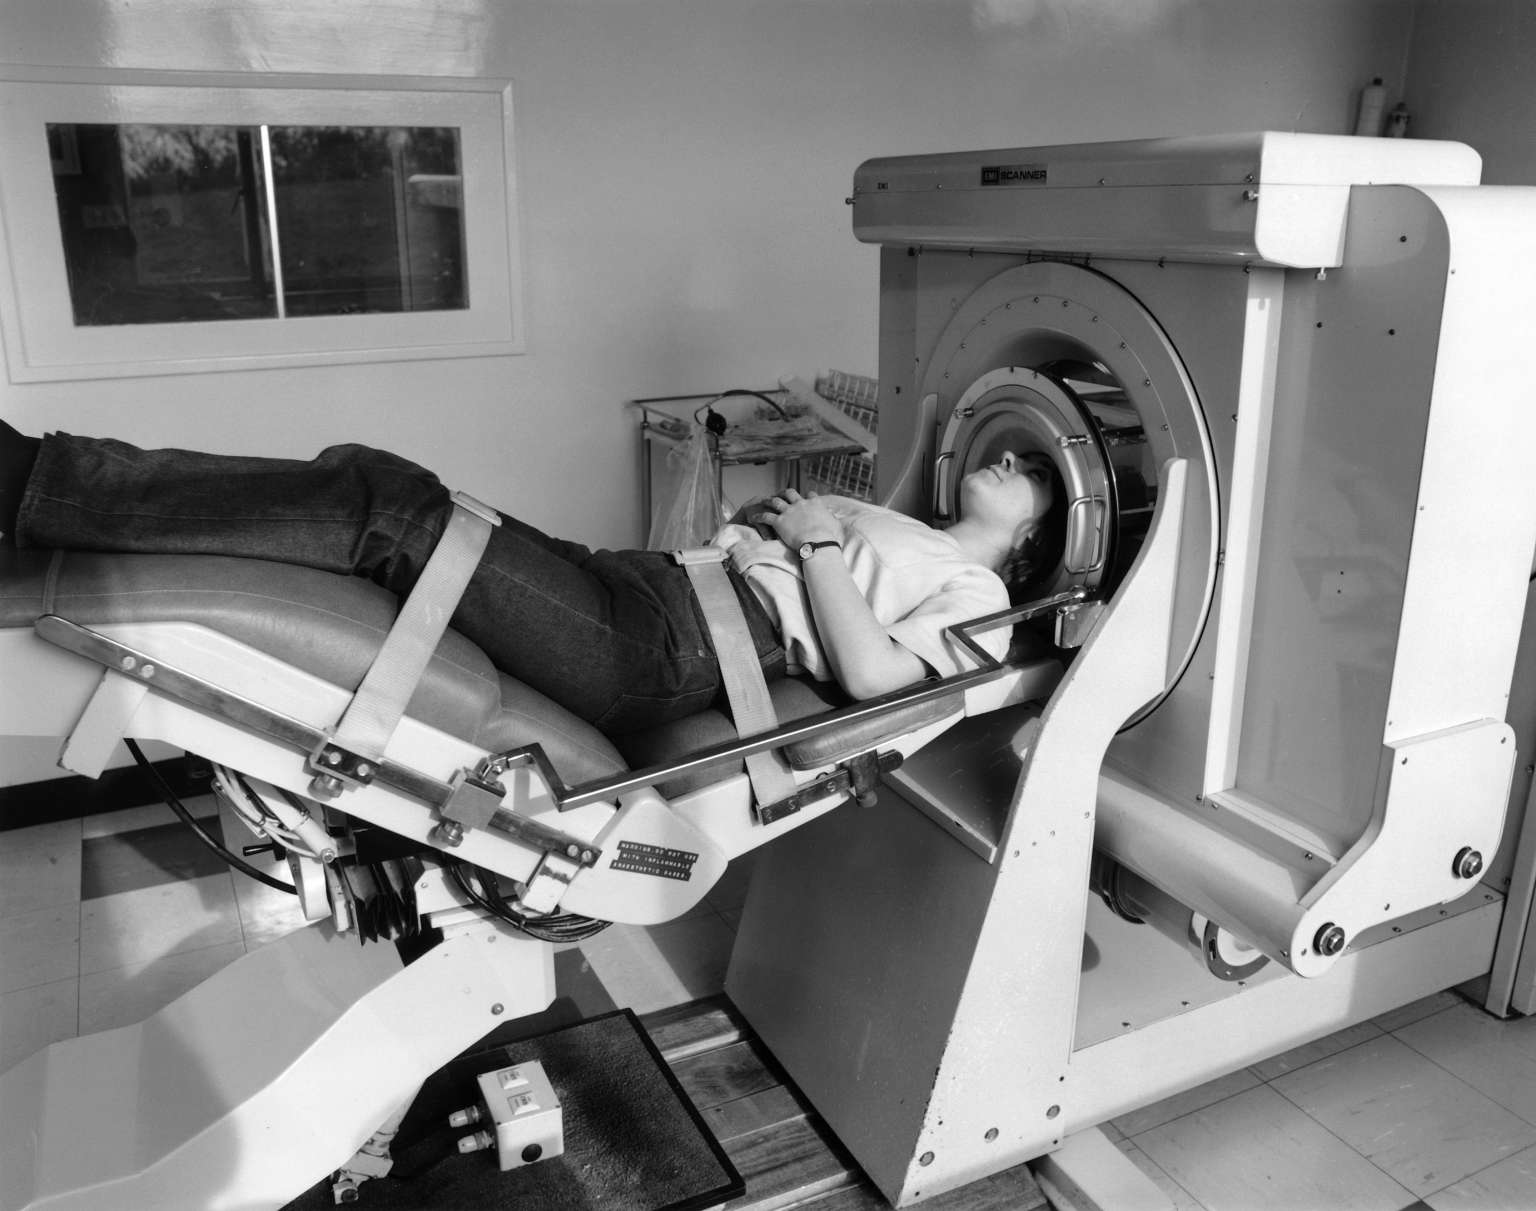
\includegraphics[width=10cm]{EMI_CT.png}
	\caption[EMI mark I]{EMI mark I sestrojený Godfrey Newbold Hounsfield v roce 1972}
\end{figure}
\null\\
CT přístroje je možné rozdělit do několika generací:
\begin{enumerate}
	\item generace - tato generace využívá tzv. Housofieldův systém, který byl použit i u přístroje EMI Mark I, snímkovací systém se v této generaci posouvá lineárně přes celou délku zkoumaného subjektu v dané rovině. Otočení je o zhruba 10$^\circ$ - 15$^\circ$. Zpracování snímků a vytvoření rekonstrukce trvalo cca 300 sec.
	\item generace - využívá stejný druh pohybu jako první generace, zmenšil se ovšem úghel mezi jednotlivými snímky na cca 3$^\circ$ - 10$^\circ$ a zvětšil se počet detektorů (až 60). Snížila se také doba rekonstrukce více než 10 a to na cca 20 sec.
	\item generace - tato generace je nejvíce využívanou variantou v současnosti. Rentgenka snímkuje objekt širokým snopcem záření za stálé rotace o 360$^\circ$. Použito je několik stovek detektorů (řádově 400-600) na protilehlé matici vůči zářiči. Snímkování se provádí po méně jak 1$^\circ$ a probíhá kontinuálně po celou dobu otořky.  \footnote[3]{Pokračováníma 3. generace je potom tzv. spirální (helikální) CT. To umožňuje postupný a plynulý posun stolu se zkoumaným objektem. Tato metoda byla poprvé použita v přístroji společnosti Bio-Imaging Research v roce 1986.}
	\item generace - Používá Rotující rentgenku, která opisuje celou kružnici záznam pak zajišťuje více než tisicovka stacionárním detekterů po obvodu. Problémem této generace je expozice okrajových detekterů, které jsou zasaženy rozptýleným a aodraženým zářením. 
	\item generace - tzv. nutační systém. ten se skládá z matice stacionárních detektorů a rotující rentgenky. Detektory se na základě pozice rentgenky vycylují z kolmice tak aby na ně paprsky dopadly kolmo. Tento systém umožňuje například rekonstrukci řezů v jiné než axiální rovině. \footnote[4]{V současné době (cca od roku 1999) vznikly i tzv. multi-slice CT. Tyto přístroje jsou vybaveny několika systémy detektorů uspořádaných do kruhu a umožňují tím pádem zísat více řezů v jednom okamžiku.Tímto způsobem ještě více urychlují vyšetření na druhou stranu stoupá jejich cena a náročnost údržby.}
	\item generace - tato generace jako zdroj záření používá elektronové dělo. Anoda je vlastně výsečí kolem čísti obvodu zkoumaného objektu a má několik ohnisek. Zařízení je buzeno současně na několika z ohniscích a detektory jsou umístěn do dvou prstenců okolo zkoumaného objektu. U této generace nedochází k žádnému pohybu. Zařízení je výše popsaným principem schopno snímkovat několik vrstev současně a to za extrémně krátkou dobu expozice, která se pohybuje okolo 50ms.
\end{enumerate}
\subsection{Princip CT}
Principem výpočetní tomografie, jak již bylo zmíněno výše je skládání celkového obrazu z mnoha jednotlivých snímků. Na následujícím obrázku je vidět, že je nutné snímkovat zkoumaný objekt z mnoha úhlů, pokud by snímkování probíhalo, jen například ze 4 nebo 6 úhlů pak by výsledný obraz byl zatížen velkou chybou.
\begin{figure}[h]
 \centering
	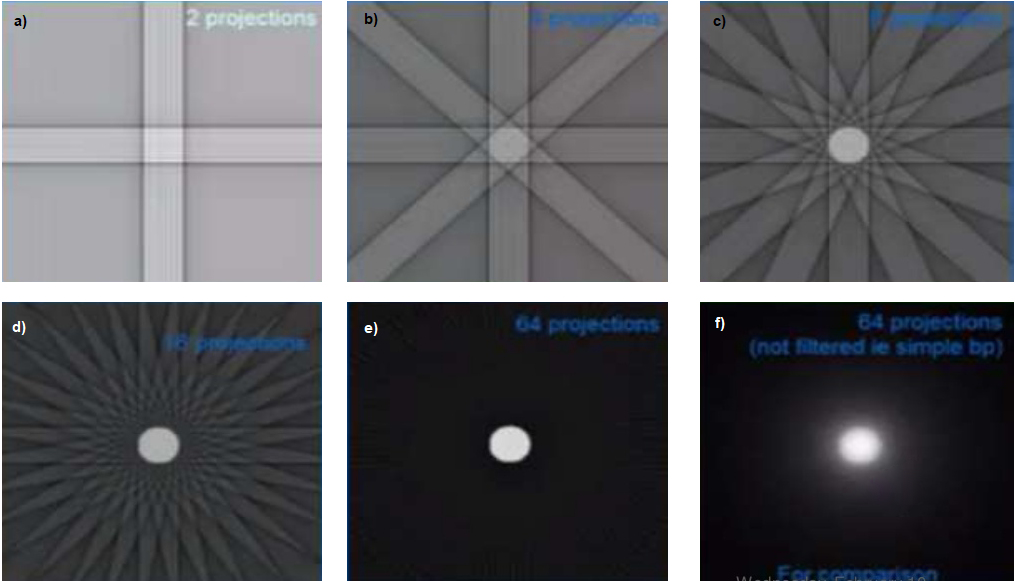
\includegraphics[width=10cm]{multiple_peojectionF.png}
	\caption[Vliv počtu projekcí na výsledný obraz]{Vliv počtu projekcí na výsledný obraz. a) 2 projekce; b) 4 projekce; c) 8 projekcí; d) 16 projekcí; e) 64 projekcí (s použitím filtru); f) 64 projekcí (bez použití filtru)}
\end{figure}
 U nejčastějšího typu CT přístrojů je rotuje rentgenka v gantře kolem pacienta a v pulzech trvajících 1-4ms vysílá vějířovitý rentgenový paprsek. Ten prochází snímkovaným objektem, kde je částečně absorbován. Po obvodu gántry jsou scintilační detektory, které zaznamenávají dopadající záření respektive míru jeho zeslabení. Tato informace je uložena do počítače a následně vyhodnocena. Obraz je potom informací o tom, jak jednotlivé voxely \footnote[5]{Voxel martix element - analogie pixelu v planárním obraze. Oproti dvojrozměrnému pixelu mají voxely ještě hloubku.}. Z pohledu medicíny je výsledkem výpočetní tomografie obraz pacienta v příčné (axiální) vrstvě, kdežto u rentgenovýh snímků vzniká obraz v frontální či sagitální vrstvě (v závislosti na poloze pacienta).\\
Absorbce rentgenového záření pro homogenní absorbér je dána následujícím vztahem:
\begin{equation}
 \centering
	I = I_{0}e^{-( \mu_{1}*x_{1} + \mu_{2}*x_{2} + ... + \mu_{y}*x_{y})}	
\end{equation}
Kde $ I_{0}$ je počáteční intezinta záření před průchodem zkoumaným objektem. $ \mu_{1}*x$ je pak součin lineárního koeficintu zeslabení $\mu$ a tloušťky homogenní části prostředí $x$. Výpočet zeslabení $I$ můžeme graficky znázornit následně:
\begin{figure}[h!]
 \centering
	\includegraphics[width=6cm]{zeslabeni_rtg_zar.png}
	\caption[Výpočet absorbce]{Výpočet zeslabení intentizi záření po prochodu absorbérem.}
\end{figure}
Nyní na jednoduchém proncipu můžeme vysvětlit na jednoduchém příkladu princip jakým je dopočítána informace pro výsledný obraz CT. Předpokládejme čtverce rozdělený na čtyři homogenní absorbéry charatkerizované zeslabením záření pro jednoduchost vyjádřeného $x_{1} - x_{4} $ s danými hodnotami. Tak jak je naznačeno na následujícím schématu:
\begin{figure}[h!]
 \centering
	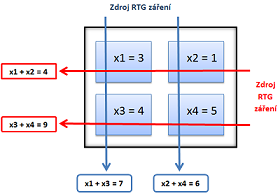
\includegraphics[width=6cm]{princip_CT.png}
	\caption[Princip výpočtu zeslabení voxelů]{Zjednodušený příklad principu výpočtu zeslabení jednotlivých voxelů}
\end{figure}
Hodnoty jednotlivých komponent $x_{1} - x_{4}$ jsou pro nás ovšem neznámou. Změřit je tedý možné jen zeslabení intentizity vždy v dané rovině (hodnoty v červených a modrých obdélnících). Díky těmto hodnotám jsme ale schopni sestavit 4 rovnice o 4 neznýámých:
\begin{equation}
 \centering
\begin{array}[h]{c}
	x_{1} + x_{2} = 4 \\
	x_{3} + x_{4} = 9 \\
	x_{1} + x_{3} = 7 \\
	x_{2} + x_{4} = 6
\end{array}
\end{equation}
Touto jednoduchou soustavou rovnic jsme pak schopni dopočítat jednotlivé parametry $x_{1} - x_{4}$. \\
Pokud se jedná o nehomogenní absorbér dostává rovnice (1) tento tvar:
\begin{equation}
 \centering
	I(x) = I_{0}(x)e^{-(\int\mu(x,y) dy) }
\end{equation}
Logaritmování tohoto vztahu dostaneme:
\begin{equation}
 \centering
\begin{array}[h!]{c}
	p(x) = -\left[\frac{I(x)}{I_{0}(x)}\right] \\
	p(x) = \int\mu (x,y) dy
\end{array}
\end{equation}
V praxi se ovšem vychází při řešení úlohy přiřazení správné hodnoty absorbce jednotlivým voxelům z tzv. Radonova transormace \footnote[6]{Autorem je Prof. Dr.phil. Johann Karl Gustav Radon narozen v Děčíne v roce 1887.} a zpětná Radonova transformace, což je integrální transformace spočívající v integrovýání funkce přes přímky. Při výpočtu CT obrazu se používá následující tvar:
\begin{equation}
 \centering
	p(r,\theta) = \int_{-\infty}^{\infty}\int_{-\infty}^{\infty} f(x,y) \delta(x cos\theta +y sin \theta - r)dx dy
\end{equation}
kde $f(x,y)$ reprezentuje $\mu (x,y) dy$ z rovnice (1), $r$ je pozice zdroje rentgenového záření a $\theta$ je úhel jeho natočení. Z tohoto vztahu je pak možné odvodit zpětnou Radonovu transformaci a s jejím použitím a využitím tzv. řezového teorému je pak možné získat dokonalý obraz pro všechny úhly. Radonova transformace se ovšem v praxi ukázala jako nestabilní a tak je v praxi nahrazena metodou filtrované projekce a Fourierova transformace.
\begin{figure}[ht!]
 \centering
	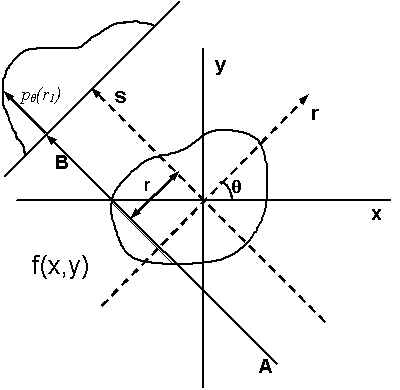
\includegraphics[width=6cm]{radonova_transformace.png}
	\caption[Radonova transformace]{Princip Radonovy transformace graficky}
\end{figure}
\subsection{Hounsfieldovy jednotky}
Hounsfieldova jednota (dále HU, někdy označované jako CT číslo) je denzintní jednotka vyjadřující míru absorpce jednoho voxelu vzhledem k refereční hodnotě absorbce vody (pro vodu HU = 0). Výpočet HU je definován následujícím vztahem:
\begin{equation}
 \centering
	HU = \frac{\mu -  \mu_{\omega}}{\mu_{\omega}}k
\end{equation}
Kde $k=10^3$ - je konstanta, $\mu$ - je koeficient zeslabení tkáně a $\mu_{\omega}$ - je koeficient zeslabení vody ( $ = 0,22cm^{-1}$). Ze vztahu (6) je patrné, že se HU je bezrozměrná veličina.\\
Rekonstruovaný CT obraz je nejčastěji zobrazován v odstínech šedi. Po provedení počítačových výpočtů je tak možné definovat rozsah zobrazovaných dat, právě rozsahem HU. Ten je pak přepoškálován a na vzniká tak grafická podoba CT snímku v odstínech šedi odpovídajících právě HU. Tímto je možné z naměřených dat analyzovat například pouze ty tkáně, na něž je vyšetření CT zaměřeno. Následující obrázek ukazuje vliv volby rozsahu na snímku plic:
\begin{figure}[ht!]
 \centering
	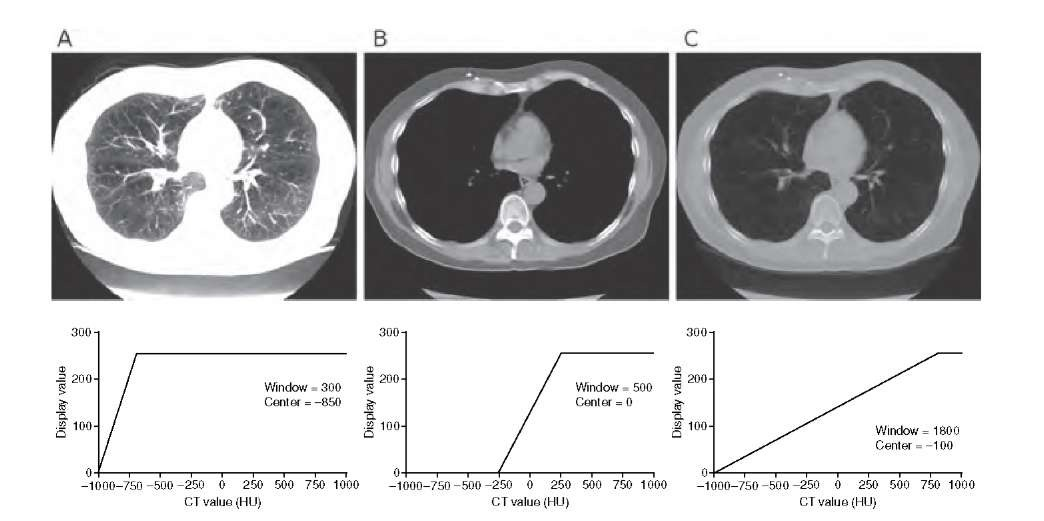
\includegraphics[width=10cm]{ruzna_HU.jpg}
	\caption[Nastavení rozsahu HU]{Nsatavení rozsahu zobrazeného HU pro CT snímek plic}
\end{figure}
V následující tabulce jsou pak zapsány přibližné hodnoty HU pro typické tkáně a orgány:\\
\begin{center}
\begin{tabular}{c|c}
 \centering
\bfseries \bfseries Tkáň & \bfseries Densita HU\\
\hline \hline
vzduch                      & -1000\\
tuk                            & -50 - (-100)\\
voda                         & 0\\
likvor                         & 5\\
bílá hmota mozková  & 30\\
šedá hmota mozková& 34\\
krev                           & 47\\
játra                          & 40 - 60\\
svaly                         & 35 - 75\\
vazivové tkáně         & 60 - 90\\
chrupavka                 & 80 - 130 \\
kost                           & 1000 - 3000 
\end{tabular}
\captionof{table}{Orientační hodnoty HU}
\end{center}
\newpage

\chapter{Formát DICOM}
Snímky z lékařských vyšetření jsou reprezontovány datovým formátem DICOM, což je zkratka anglického \textbf{Digital Imaging and Communications in Medicine}. Jedná se o standart pro zobrazování a také skladování dat například z MRI nebo CT vyšetření. DICOM byl vytvořen v roce 1993 výborem \textbf{DICOM Standard Committee}\footnote[7]{První verze ACR/NEMA 300 byla uvolněna 1985. Následovala ARC/NEMA 2.0. V současné době je platný DICOM 3.0 z roku 1993} a jeho autorská práva vlastní asociace  \textbf{NEMA} (National Electrical Manufacturers Association)\footnote[8]{NEMA se rozhodla po zavedení výpočetní tomografie v 70. letech vytvořit v roce 1983 výbor pro nalezení standartu na přenos snímků a přidružených informací.}. Tento standart definuje způsob práce s daty a to například sdílení, mazání a jejich ukládání. Slouží také pro definici tisku, skenovaní a integraci do systému \textbf{PACS} (Picture Archiving and Communication System).
 \begin{figure}[htp!]
  \centering
	
\includegraphics[width=4cm]{dicom.jpg}
	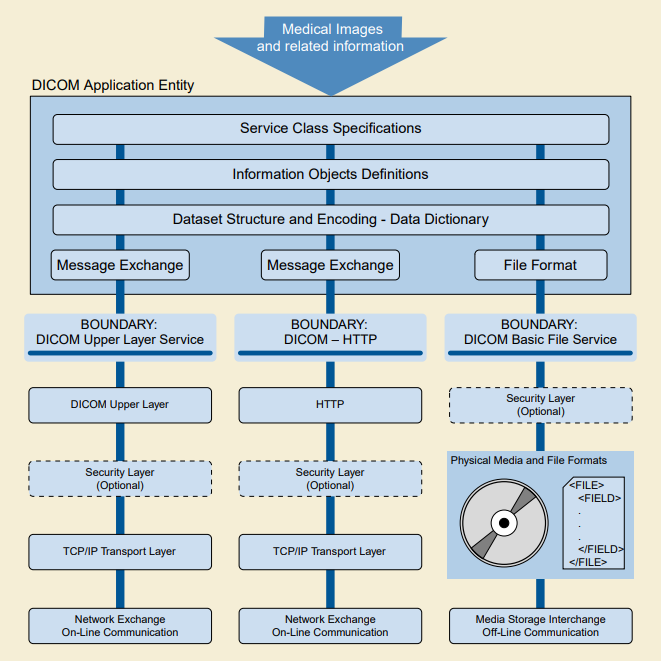
\includegraphics[width=6cm]{dicom_genmod.png}
	\caption[DICOM]{Obecné komunikační schéma DICOM}
\end{figure}
\null\\
Pro tuto práci je ovšem důležité že data úkladaná standartem DICOM, neobsahují pouze vlastní obrazová data, ale mnoho metadat. Jsou to například informace o pacientovi, průběhu a typu vyšetření, datu, kdy bylo vyšetření provedeno a pro tuto práci podstatné informace o měřítku. Jednotlivé datové soubory obsahují informace o tom, jak každý pixel v jednotlivých směrech odpovídá skutečnému rozměru.


\chapter{Příprava obrazových dat}

\section{Histogram equalization}
Do češtiny je možné název této metody přeložit jako ``vyrovnání histogramu'' více se ale používá anglický název. Jedná se o metodu, která upravuje kontrast obrazu. Algoritmus je definován následujícím vztahem:
\begin{equation}
 \centering
 T^{*} = argmin_{T}(|c_{1}(T(k)) - c_{0}(k)|)
\end{equation}
kde $c_{0}$ je požadovaný kumulativní histogram. Na obrázcích níže je vidět jak metoda funguje. Na obráztku b) je patrné, že původně velmi úzký jasový histogram se po použití metody ``roztáhne''. Z principu této metody plyne i její použití především na obrazových datech s nízkým kontrastem.
 \begin{figure}[htp!]
  \centering
  
   \begin{minipage}[c]{\textwidth}
	\centering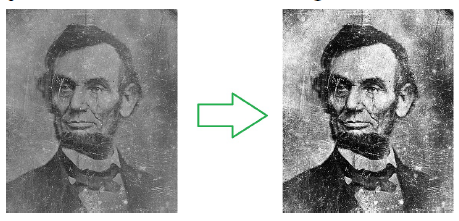
\includegraphics[width=3.5cm]{histeq.png}\\
     a)
   \end{minipage}
    \begin{minipage}[c]{\textwidth}
	\centering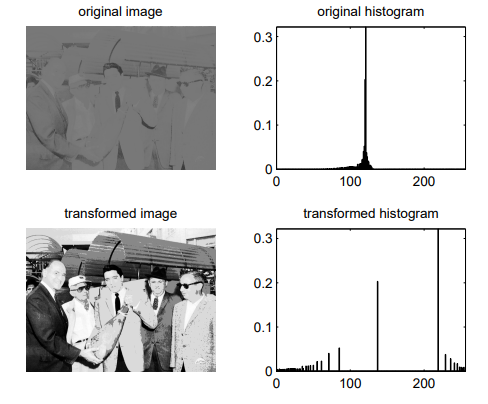
\includegraphics[width=3.5cm]{histeq2.png}\\
     b)
   \end{minipage}

	\caption[Histogram equalization]{Histogram equalization}
\end{figure}
\newpage
\section{CLAHE}
CLAHE = Contrast Limited Adaptive Histogram Equalizetion. Tuto metodu nejlépe popisuje následující obrázek, který vyjadřuje jak se pracuje s histogramem:
 \begin{figure}[htp!]
  \centering
  
   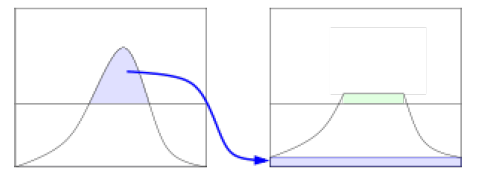
\includegraphics[width=4cm]{clahe.png}\\ 
    \caption[CLAHE]{Contrast Limited Adaptive Histogram Equalizetion}
\end{figure}
V podstatě jde o předpoklad, že v obraze nemůže být žádná hodnota jasu zastoupena s četností vyšší než je definovaná prahová hodnota. Pokud tedy jas v histogramu tuto hranici překročí, je hodnota oříznuta a tato část je rozložena mezi ostatní jasy rovnoměrně. Ukázka CLAHE je patrná na následujícím obrázku:
 \begin{figure}[htp!]
  \centering
   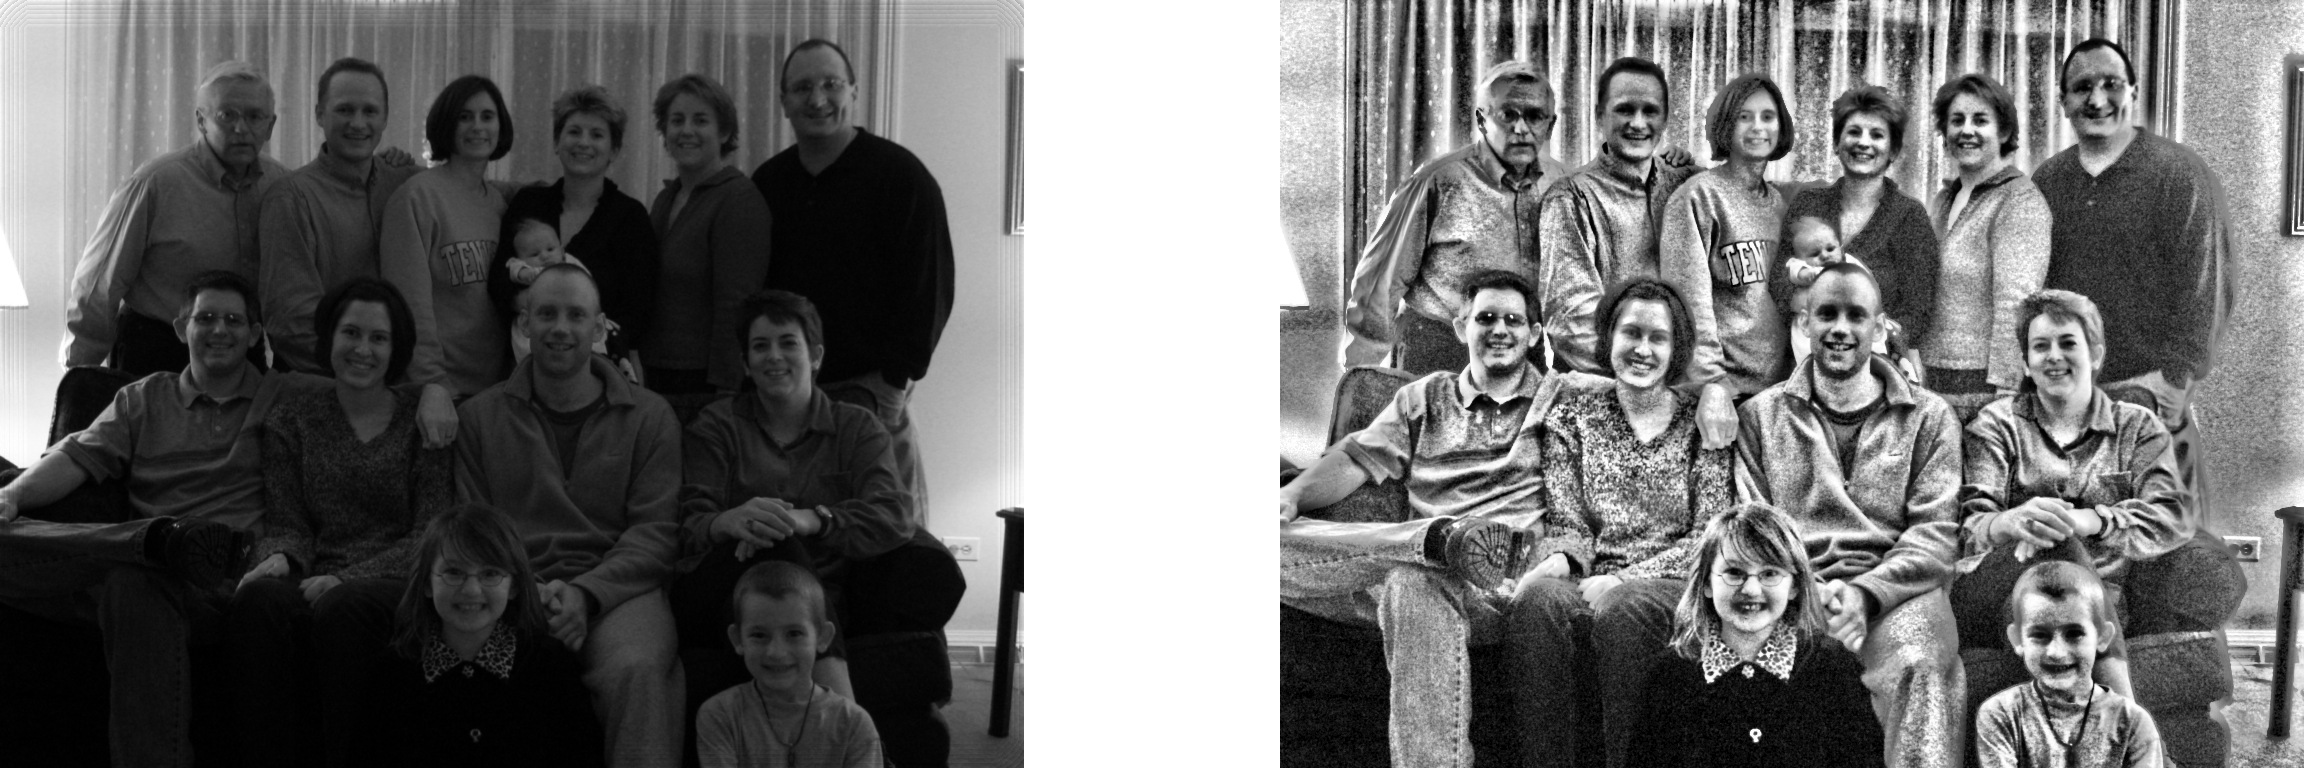
\includegraphics[width=7cm]{clahe2.png}\\ 
    \caption[CLAHE ukázka]{Ukázka metody Contrast Limited Adaptive Histogram Equalizetion}
\end{figure}
\section{Vyhlazování}
Většina obrazových dat, kterou chceme zpracovat je zatížená šumem, samozřejmě se jedná i o případ snímků z CT. Tento šum může mít za následk mnohé problémy například při segmentaci a potažmo i při registraci obrazových dat. Cílem přípravy obrazových dat je tedy tento šum v idálním případě zcela odstranit, což ovšem není v podstatě možné, a tak se cílem obrazový šum alespoň minimalizovat.\\

\subsection{Konvoluce}
Myšlenka vyhlazovaní v obraze pro případ šumu se opírá o možnost upravit hodnotu pixelu na základě analýzy malého okolí. Jedním z prostředků odstranění šumu je rozmazání. Nevýhodou tohoto přístupu je skutečnost, že ztrácíme určitou míru informace z obrazu a problémem bývají také ostré jasové přechody. \\
Pro vyhlazování se často používá diskrétní 2D konvoluce. Můžeme jí zapsat následující rovnicí:
\begin{equation}
g(x,y) = \sum_{m,n}h(x-m,y-n) f(m,n)
\end{equation}
kde $h$ je konvoluční maska, která udává váhu hodnot obrazové funkce daného okolí. Velmi často se používá obdélníkové nebo čtvercové okolí bodu. Nejjednoduším případem konvoluce je prosté průměrování za použití konvoluční masky:
$$
h = 1/9
\left[
\begin{matrix}
1&1&1\\
1&1&1\\
1&1&1
\end{matrix}
\right]
$$

 Tato konvoluční maska je pak postupně přikládána na jednotlivé pixely obrazy a je dopočítána nová hodnota jasu pixelu, která pro tuto konkrétní masku $h$ je obyčejným aritmetickým průměrem osmiokolí bodu. Princip konvoluce je graficky naznačen i na následujícím obrázku:
   \begin{figure}[htp!]
  \centering
   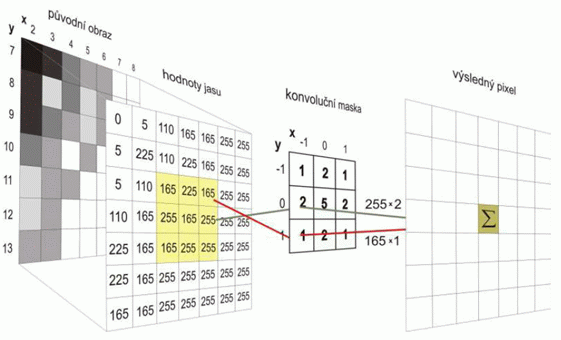
\includegraphics[width=7cm]{konvoluce.png}\\ 
    \caption[Konvoluce]{Konvoluce}
\end{figure}
Konvoluční maskou může být v podstatě jakkákoliv matice. Následující konvoluční masky napířklad přidávají význam pixelům blíže středu masky:
$$
h =\frac{1}{10}
\left[
\begin{matrix}
1&1&1\\
1&2&1\\
1&1&1
\end{matrix}
\right];
h =\frac{1}{16}
\left[
\begin{matrix}
1&2&1\\
2&4&2\\
1&2&1
\end{matrix}
\right];
h =\frac{1}{50}
\left[
\begin{matrix}
1&1&3&4&3&1&1\\
1&2&4&8&4&2&1\\
1&1&3&4&3&1&1
\end{matrix}
\right]
$$

\subsection{Gaussův filtr}\label{gauss}
Tato metoda skládá konvoluční masku z prvků, které jsou určeny Gaussovou funkcí tedy normálním rozdělením. Je to velmi často používaná metoda, jejímž hlavním nedostatkem je rozmazání obrazu. Maska Gaussova filtru má tedy prvky vypočtené následující rovnicí:
 \begin{equation}
 G(x,y) = \frac{1}{2\pi\sigma^2}e^{-\frac{x^2+y^2}{2\sigma^2}}
 \end{equation}
 kde $\sigma$ je směrodatná odchylka. Příklad konvoluční masky $h$ pro velikost $5x5$': 
$$
h = \frac{1}{273}\left[
\begin{matrix}
1&4&7&4&1\\
4&16&26&16&4\\
7&26&41&26&7\\
4&16&26&16&4\\
1&4&7&4&1
\end{matrix}
\right]
$$
\subsection{Metoda rotující masky}
Máme-li konvoluční masku, je možné také použít metodu rotující masky. Mějme například masku o rozměru $3x3$ pro daný pod se maska posouvá, tak že zkoumaný bod je vždy na jiné pozici masky. Místo prostého osmiokolí je tak zkoumáno okolí o rozměru $5x5$ tak jak je naznačeno na následujícím schématu:
   \begin{figure}[htp!]
  \centering
   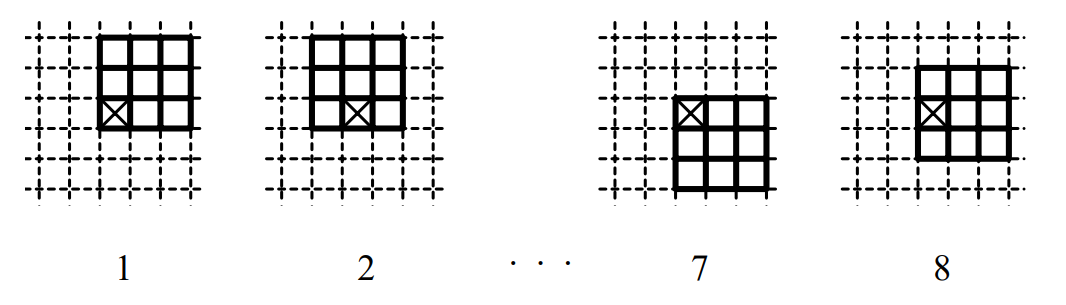
\includegraphics[width=7cm]{rotmask.png}\\ 
    \caption[Metoda rotující masky]{Metoda rotující masky}
\end{figure}
Celkem je tedy možných 9 poloh konvoluční masky vůči zkoumanému bodu. Vybraná pro vlastní výpočet je následně ta, která má nejmenší rozptyl.
\subsection{Nelinéární filtry}
\subsubsection{Mediánový filtr}
Medián je tzv 2-kvantil, tedy hodnota daná stejně velkýmni intervaly z kumulativní distribuční funkce náhodné veličiny. Obecně tedy $q-kvantil$ rozdělí data do $q$ stejně velkých částí. Mějme tedy data $X$  a hodnotu $M$ pak pravděpodobnost $x\in X: x<M$ je rovna pravděpodobnosti jevu $x \in X : x>M;$ hodnotu $M$ pak nazýváme medián. V obrazovém vyhlazovaní se jedná o to, že se opět vezme $n$-okolí zkoumaného bodu. Hodnoty pixelů se seřadí vzestupně (může být i sestupně) a medián se určí jako prvek, který je uprostřed dané řady. Typické je použití takové matice (resp. okolí bodu), která má lichý počet prvků ($3x3; 5x5$). Výpočet je v tomto případě velmi rychlý, což je hlavní výhodou mediánové filtrace\footnote[9]{Výpočet je možné ještě urychlit tím, že posloupnost stačí být uspořádaná pouze částečně}, dále je výhodou značná robustnost. Naopak nevýhodou je skutečnost, že v obdélníkovém okolí porušuje tenké čáry a ostré hrany 
\subsubsection{Konzervativní vyhlazení}
Tento filtr slouží především k odfiltrování izolovaných pixelů s výjimečně vysokou nebo nabo nízkou intenzitou. Nalezneme tedy minimum a maximum v okolí bodu a pokud je hodnota v rozmezí definovaném zmíněným rozsahem je ponechána. Pokud je hodnota pod minimem, je nahrazena hodnotu právě minima a analogicky tato úvaha platí pro překročení maxima okolí bodu. Tento typ je vhodný především pro odstranění šumu typu ``sůl'' nebo ''rýže'' 
\subsubsection{Prahování vlnkových koeficientů}
Nejprve je spočítána hodnota jednotlivých bodů pomocí diskréní vlnkové transformace a dále se volí buď tvrdé prahování:
$$
\rho_{\lambda}^{tvrdé}(x)\Bigg\{
\begin{matrix}
x\;&\;|x|\geq\lambda\\
\null&\null\\
0\;&\;|x|<\lambda
\end{matrix}
$$
nebo měkkého
$$
\rho_{\lambda}^{měkké}(x)\Bigg\{
\begin{matrix}
x-\lambda\;&\;x\geq\lambda\\
x+\lambda\;&\;x\leq -\lambda\\
0\;&\;|x|<\lambda
\end{matrix}
$$
\subsubsection{Bilaterální filtr}
Metoda\footnote[10]{Bilaterální filtr byl prezentován až v roce 1998 dovjicí Tomasi a Manduchi}, která vykazuje velmi dobré výsledky, ovšem to je kompenzováno časovou nároční.  Hlavní výhodou je že zachovává významné jasové přechody (hrany) v obraze a naopak filtruje šum na souvislých plochách. Filtr pracuje na principu průměrovaní hodnot bodu pouze z okolních bodů s podobnou hodnotou. Pro body s nízkou jasovou hodnotou uvažuje pro průměrování pouze body s podobně nízkými jasovými hodnotami a tím tmavá místa nezesvětluje a zachovává ostrost hrany. \footnote[11]{V barevném prostoru je nutné převést obraz do barevného prostoru CIE-LAB. Nepostačují totiž pouze tři kanály RGB reprezentace.}
\subsection{Ukázka použití některých filtrů}

 \begin{figure}[htp!]
  \centering
  
   \begin{minipage}[c]{0.4\textwidth}
	\centering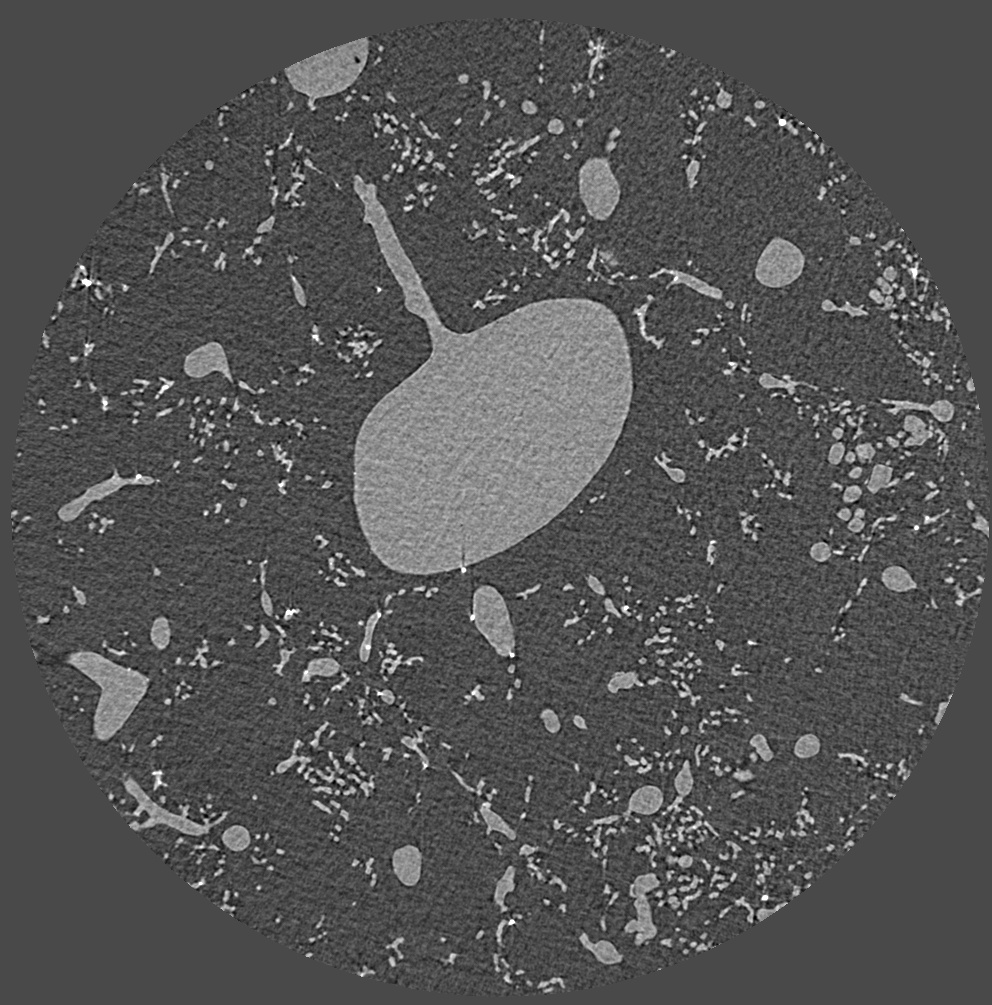
\includegraphics[width=5cm]{bluring/origImg.jpg}\\
     a)
   \end{minipage}
   \hspace*{0.5cm}
    \begin{minipage}[c]{0.4\textwidth}
    
	\centering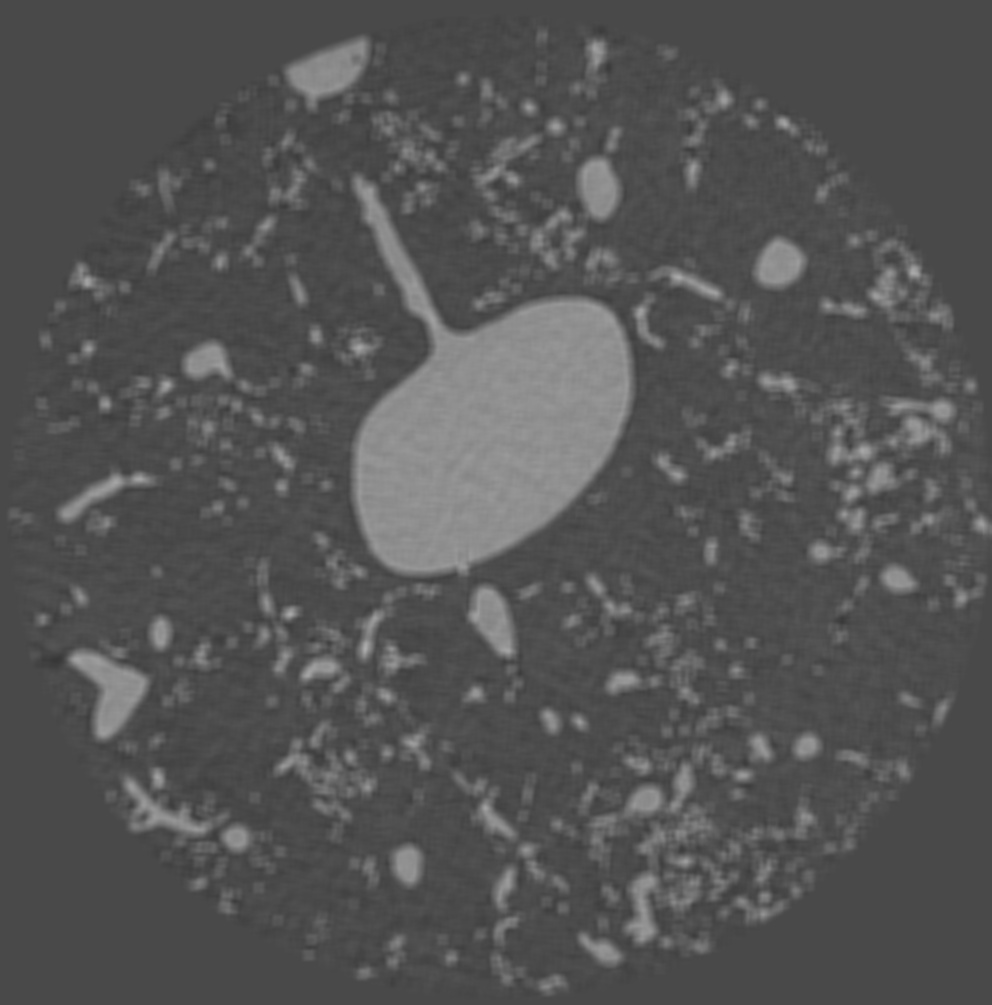
\includegraphics[width=5cm]{bluring/convImg.jpg}\\
     b)
   \end{minipage}
    \begin{minipage}[c]{0.4\textwidth}
	\centering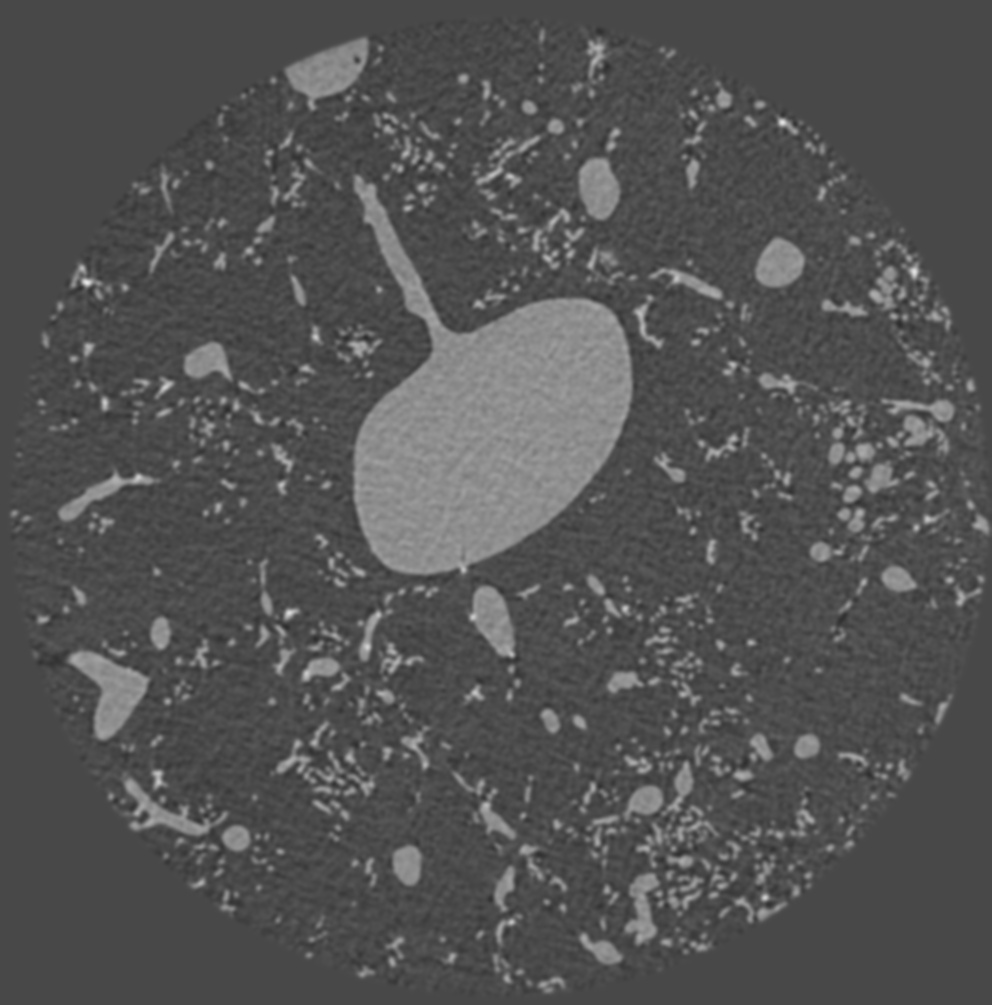
\includegraphics[width=5cm]{bluring/gaussImg.jpg}\\
     c)
   \end{minipage}
\hspace*{0.5cm}
    \begin{minipage}[c]{0.4\textwidth}
	\centering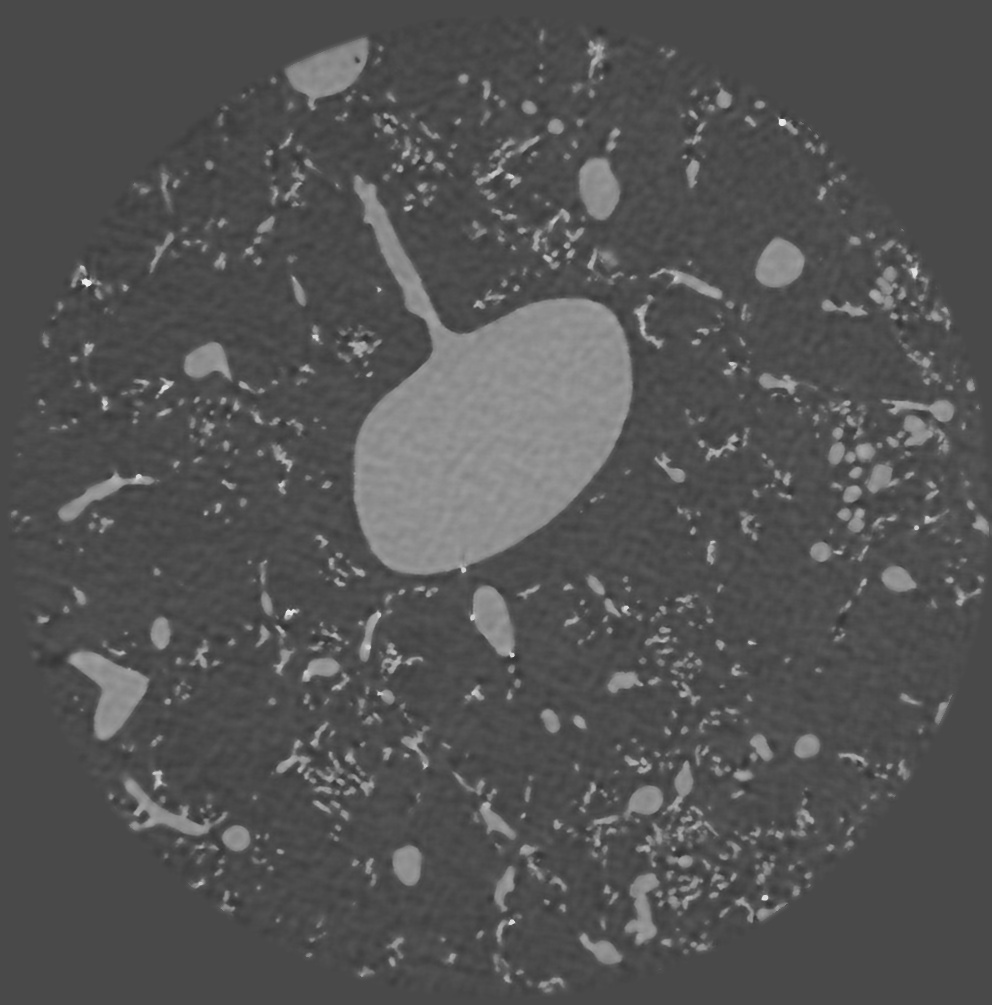
\includegraphics[width=5cm]{bluring/bilImg.jpg}\\
     d)
   \end{minipage}
    \begin{minipage}[c]{\textwidth}
	\centering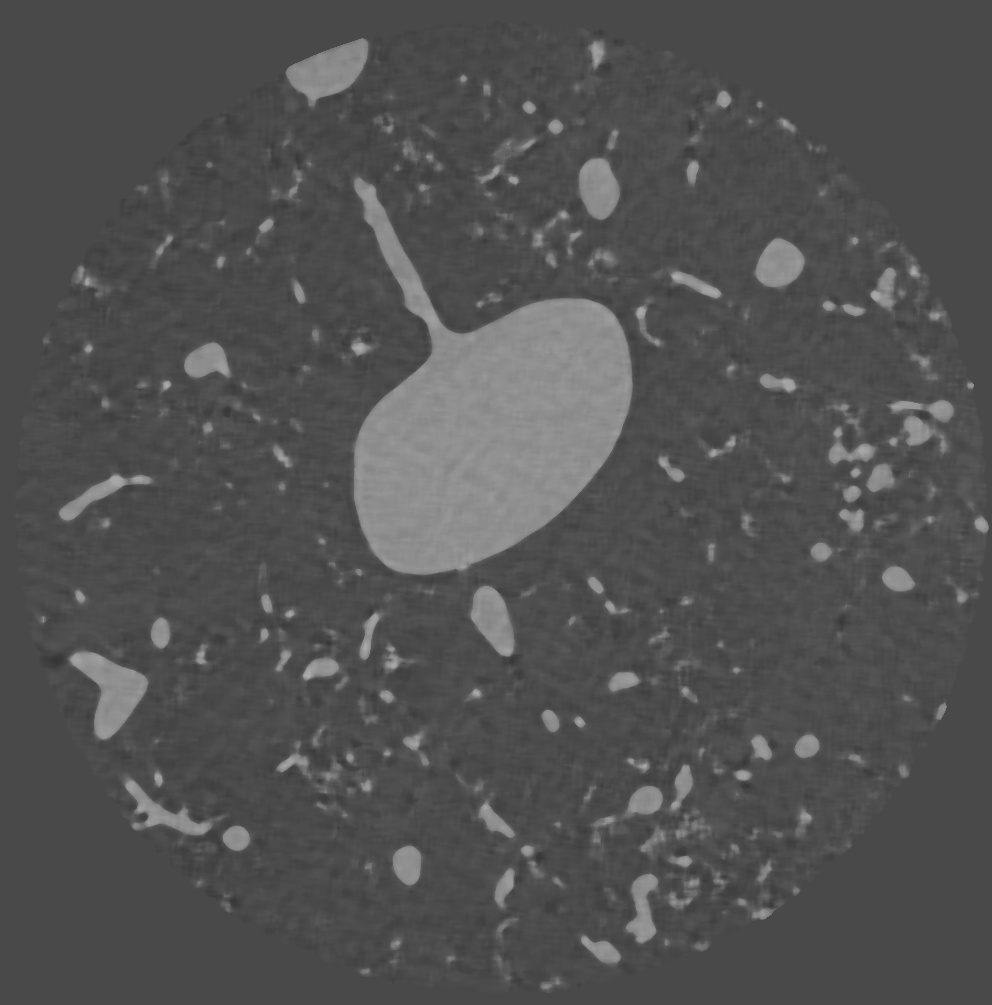
\includegraphics[width=5cm]{bluring/medImg.jpg}\\
     e)
   \end{minipage}

	\caption[Vyhlazování šumu]{Vyhlazování šumu - a) původní obraz; b) průměrování; c) Gaussův filtr; d) bilaterální filter; e) medián pro masku velikosti 11x11}
\end{figure}
%Výpočet času pro jednotlivé metody
\begin{center}
\begin{tabular}{l|c|c}
 
\bfseries \bfseries Metoda & \bfseries Velikost masky & \bfseries Čas/sec\\
\hline \hline
Průměrování &11x11             & 44.01\\
Průměrování &3x3                 & 6.58\\
Gaussův filtr &11x11              & 6.60\\
Gaussův filtr &3x3                  & 6.71\\
Medián &11x11                       &19.12\\
Medián &3x3                           &7.01\\
Bilaterální filtr &11x11            &43.14\\
Bilaterální filtr &3x3                &10.95\\
\end{tabular}
\captionof{table}{Časová náročnost pro jednotlivé metody}
\end{center}
Pozn.: Časy jsou měřeny pro MakroCT snímky. Cca 750 snímků o celkové velikosti 380MB.
\newpage
\section{Segmentace}
Segmentace slouží k rozdělení obrazu na několik částí (segmentů) které mají společné vlastnosti. Metod, které se dají za tímto účelem je celá řada, některé jsou popsány v následujicích kapitolách cílem bývá často najít na obraze nějaký konkrétní objekt nebo například identifikovat popředí a pozadí. Kromě zpracování snímků v oblasti medicíny se segmentace používá například při dálkovém průlzkumu země nebo trekovaní objektů na snímcích kamer.\\
Segmentaci obrazu můžeme zapsat pro $\mathbb{R}^2$ prostor ve kterém mějme obraz $f(x,y)$  jako rozdělení na $R_{orig}$ na $R_{1},R_{2},...,R_{n}$ částí, které splňují následující kritéria:

\begin{enumerate}
	\item $\bigcup_{i=1}^n R_{i} = f(x,y)$
	\item $R_i \uplus R_j = \emptyset, i \neq j$
	\item $\forall f(x,y), x,y \in R_{i}; f(i,j), i,j \in R_{i}: f(x,y) =  f(i,j)\pm \alpha$, kde $\alpha$ je rozsah hodnot pixelů v daném segmentu \footnote[12]{Podmínku 3) je možné zapsat i jinými způsoby, dle typu segmentace.}
\end{enumerate}
\subsection{Prahování}
Prahování (anglicky \textit{thresholding}) je metoda, ve které jsou jasové hodnoty vyšší než definovaný práh považovány za popředí obrazu a všechny body s hodnotou jasu nižší naopak za pozadí. Jedná se tedy o jasovou transformaci vstupního obrazu $f$ na výstupní binární obraz $g$. Mějme prahovou hodnotu $T$ potom:
\begin{equation}
g(i, j) = \bigg\{ 
\begin{matrix}
1\;&\;f(x,y)\geq T\\
0\;&\;f(x,y)< T
\end{matrix}
\end{equation}
Obecně je možné zavést nikoliv jeden práh $T$ ale několik prahů pro jeden obraz pak za předpokladu $T_1<T_2<T_3<...<T_m$ platí:
\begin{equation}
g(i, j) = \Bigg\{ 
\begin{matrix}
n\;&\;f(x,y)\ \geq T_m \\
... &\;\\
2\;&\;f(x,y)\ \geq T_2 \wedge f(x,y) < T_3 \\
1\;&\;f(x,y)\ \geq T_1 \wedge f(x,y) < T_2 \\
0\;&\;f(x,y)< T_1
\end{matrix}
\end{equation}
Dále je možné uvažovat i prahování jednostranné nebo oboustranné. Pro dvě prahové hodnoty platí u oboustraného prahovaní, že prahovaný obraz bude mít hodnotu jedna pouze pokud je hodnota jasu mezi danými hranicemi. Jinak bude hodnota výsledného obrazu 0.\\
\subsubsection{Non-maximal supression} \label{nonMaxSup}
Důležitým aspektem úspěšného použití prahování při segmentaci obrazu je určení prahové hodnoty, ta se často získává na základě analýzy histogramu. Metoda non-maximal supression (česky \textit{potlačení nemaxim}) je rychlou a účinnou metodou nalezení lokálních maxim. Ta je pak možné využít právě k určení prahové hodnoty. Jak metoda funguje je patrné na následujícím schématu:

 \begin{figure}[htp!]
  
	\centering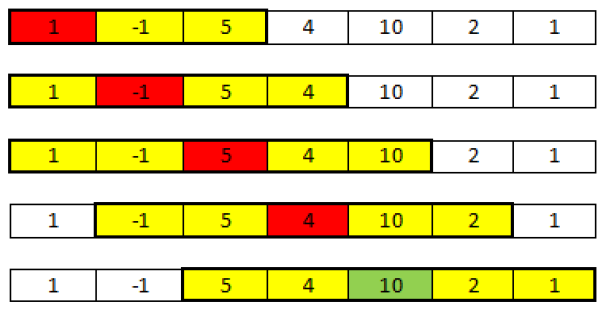
\includegraphics[width=7cm]{nonmaxsup.png}\\
	\caption[Non-maximum supression]{Non-maximum supression}
\end{figure}
Metoda po zkoumaném obraze (histogramu) posouvá okénko a dívá se jestli je bod v centru maximem v rámci okolí. Pokud ne posouvá okénko dále. Pokud ano, metoda označuje tento bod za lokální maximum. Zřejmou nevýhodou je potřeba mít dostatečně velké okénko.

 \begin{figure}[htp!]
  \centering   
  \begin{minipage}[c]{\textwidth}
	\centering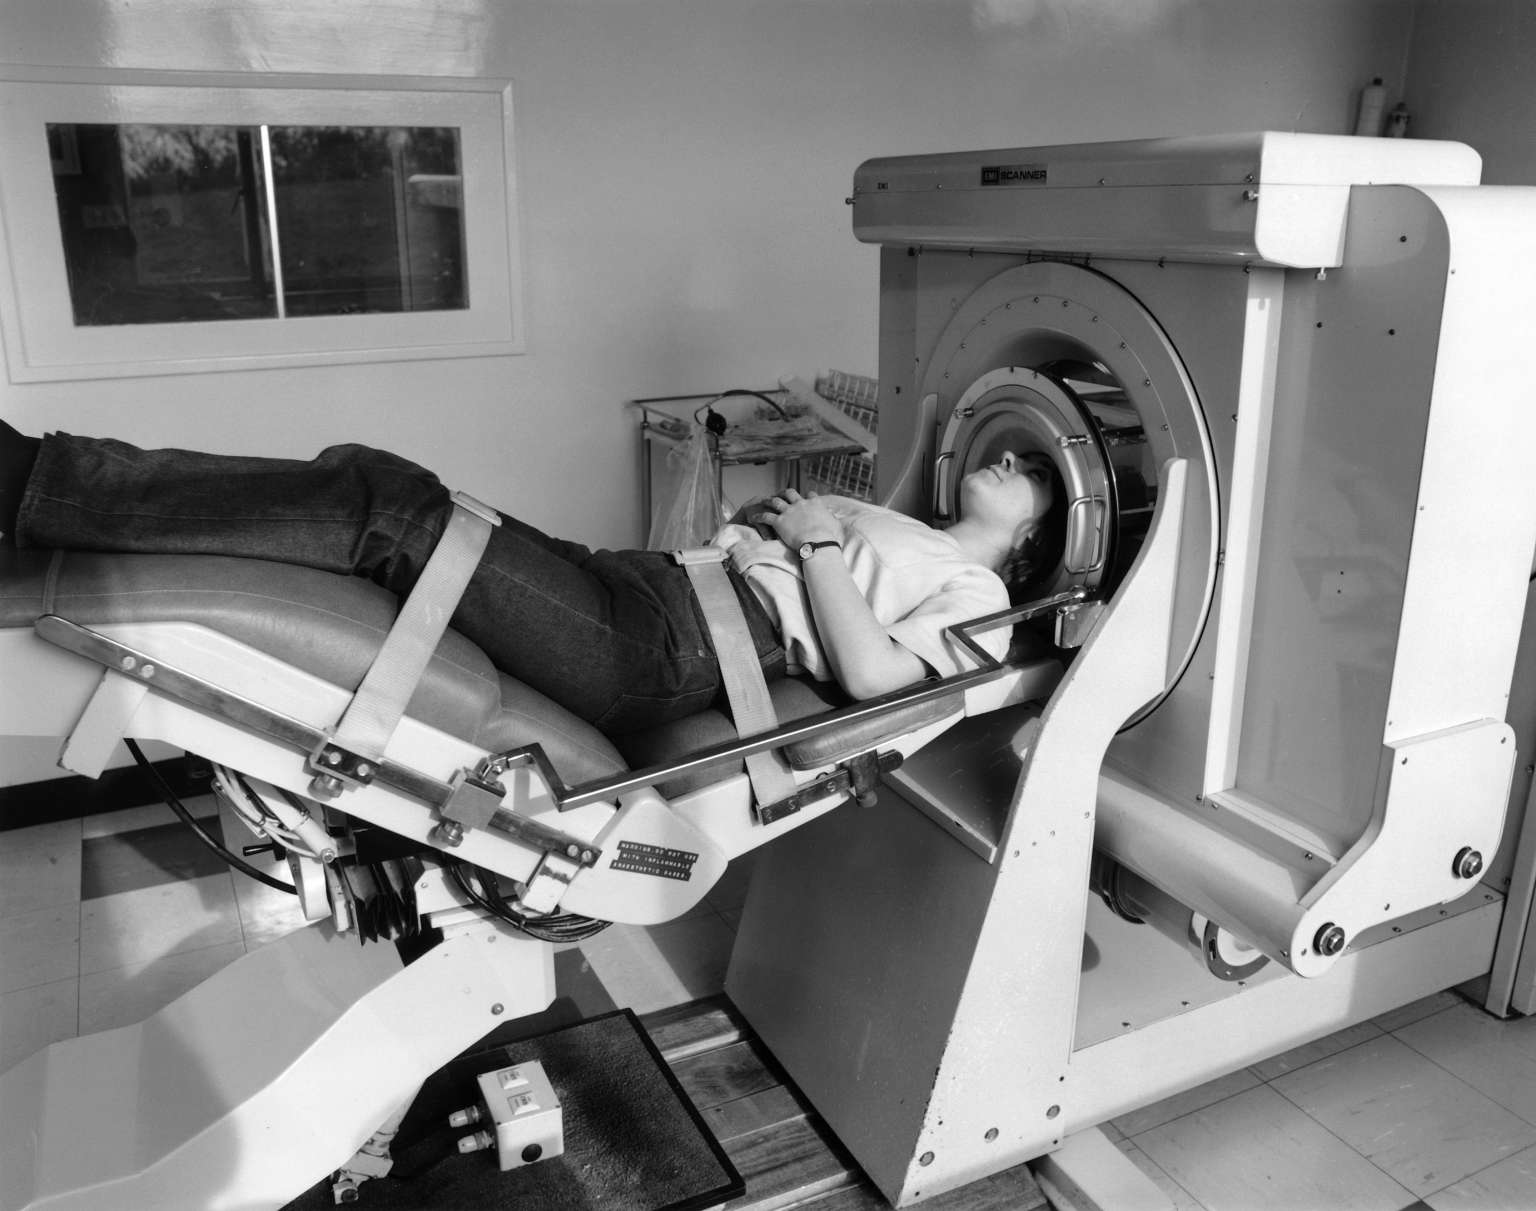
\includegraphics[width=3cm]{EMI_CT.png}\\
     a)
   \end{minipage}
  
   \begin{minipage}[c]{0.3\textwidth}
	\centering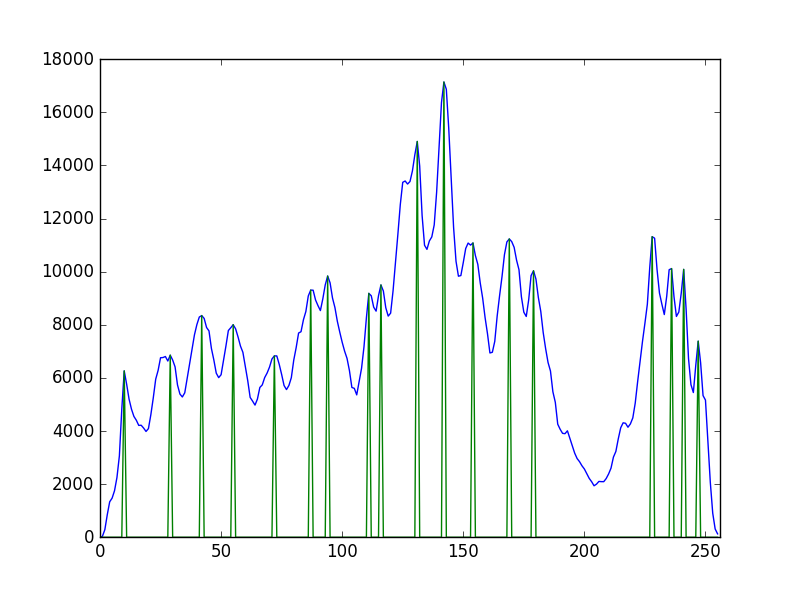
\includegraphics[width=4cm]{figNonMaxSup/tooShort.png}\\
     a)
   \end{minipage}
   \hspace*{0.1cm}
    \begin{minipage}[c]{0.3\textwidth}
    
	\centering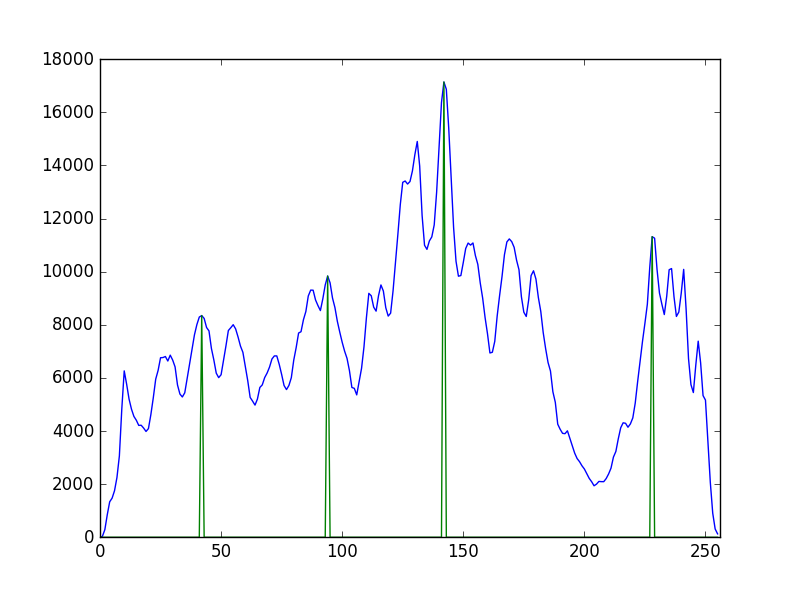
\includegraphics[width=4cm]{figNonMaxSup/val50.png}\\
     b)
   \end{minipage}
   \hspace*{0.1cm}
    \begin{minipage}[c]{0.3\textwidth}
	\centering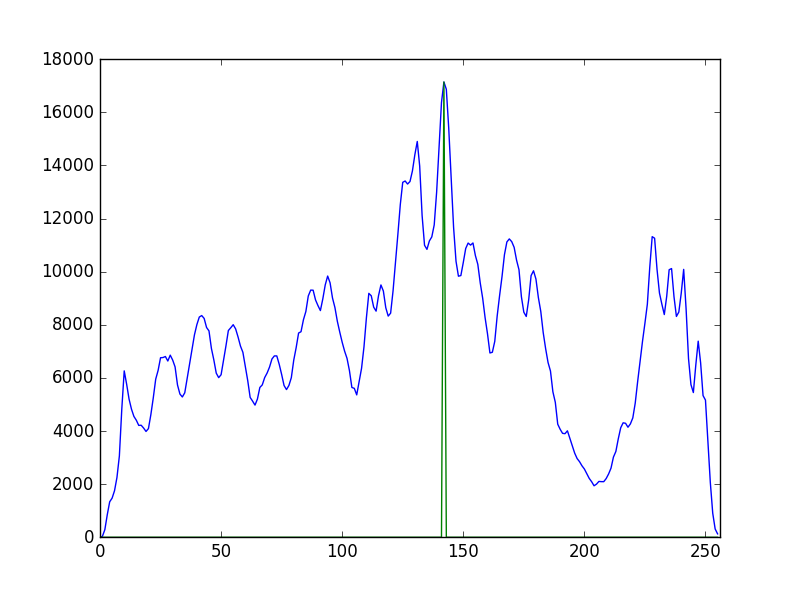
\includegraphics[width=4cm]{figNonMaxSup/tooLong.png}\\
     c)
   \end{minipage}

	\caption[Non maximum supression ukázka]{Non maximum supression s vyznačenými maximy v histogramu pro a) příliš malé okénko - velmi mnoho lokálním maxim; b) rozumnou hodnotu c) příliš velké okénko- pouze jedno lokální maximum = globální maximum}
\end{figure}

 \subsubsection{Adaptivní prahování}
 Adaptivní prahování je realizováno tak, že je práh funkcí polohy v obraze, jinými slovy můžeme říct, že je práh určován vždy pro část obrazu. Podobně jako u předešlé metody je nezbytné správně určit velikost oblasti, pro níž je práh určován. V případě že jsou jednotlivé části disjuktní může docházet ke vzniku nežádoucích artefaktů na přechodech jednotlivých oblastí. Tento problém se dá řešit buďto částečným překryvem oblastí, interpolací nebo počítat pro oblast kolem každého obrazového bodu (tato možnost vede na velkou časovou náročnost).\\
 Metoda adaptivního prahování se využívá například pro obrazová data s nevyrovnanými jasovými oblastmi, ty mohou vzniknout například nerovnoměrným osvětlením snímaného objektu.
\subsubsection{Otsu}
Metoda slouží k nalezení ideální hodnotu prahu pro bimodální histogram\footnote[13]{Metoda pojmenována po japonském matematikovi jménem Nobuyuki Otsu}. Předpokládá tedy dva vrcholy histogramu a práh se pak hledá takový, který minimalizuje vážený rozptyl $\sigma_W$  dvou jasových tříd. Ekvivaletně je možné zapsat jako maximalizaci rozptylu jednotlivých tříd. Mějme tedy dvě třídy $C_0 \in {1,2,3,...,k}, C_1 \in {k+1, ...,L}$ potom
\begin{equation}
p_i = \frac{n_i}{N}, p_i \geq 0,  \sum\limits_{i=1}^Lp_i = 1
\end{equation}
\begin{equation}
\omega_0 = Pr(C_0) =  \sum\limits_{i=1}^k p_i =\omega(k)
\end{equation}
\begin{equation}
\omega_1 = Pr(C_1) =  \sum\limits_{i=k+1}^L p_i =1-\omega(k)
\end{equation}
nyní definujme průměry obou skupin:
\begin{equation}
\mu_0 =  \sum\limits_{i=1}^k iPr(i|C_0) = \sum\limits_{i=1}^k \frac{ip_i}{\omega_0} = \frac{\mu(k)}{\omega(k)}
\end{equation}
\begin{equation}
\mu_1 =  \sum\limits_{i=k+1}^L iPr(i|C_1) = \sum\limits_{i=k+1}^L \frac{ip_i}{\omega_1} = \frac{\mu_T - \mu(k)}{1-\omega(k)}
\end{equation}
a celkový jasový průměr:
\begin{equation}
\mu_T = \mu(L) = \sum\limits_{i=1}^L iP_i
\end{equation}
Nyní definujme variace pro obě skupiny:
\begin{equation}
\sigma_0^2 = \sum\limits_{i=1}^k (i-\mu_0)^2Pr(i|C_0) = \sum\limits_{i=1}^k(i-\mu_0)^2\frac{p_i}{\omega_0}
\end{equation}
\begin{equation}
\sigma_1^2 = \sum\limits_{i=k+1}^L (i-\mu_1)^2Pr(i|C_1) = \sum\limits_{i=k+1}^L(i-\mu_0)^2\frac{p_i}{\omega_1}
\end{equation}
dále platí:
\begin{equation}
\omega_0\mu_0+\omega_1\mu_1=\mu_T
\end{equation}
\begin{equation}
\omega_0+\omega_1 = 1
\end{equation}
Nyní zapišme kritérium optimality které vychází z diskriminační analýzy:
\begin{equation}
\lambda = \frac{\sigma_B^2}{\sigma_w^2}; \; \kappa = \frac{\sigma_T^2}{\sigma_w^2}; \; \eta= \frac{\sigma_B^2}{\sigma_T^2}
\end{equation}
pro $\sigma_T^2, \sigma_w^2$ a $\sigma_B^2$ platí:
\begin{equation}
\sigma_w^2 = \omega_0\sigma_0^2 + \omega_1\sigma_1^2
\end{equation}
\begin{equation}
\sigma_B^2 = \omega_0(\mu_0-\mu_T)^2+\omega_1(\mu_1-\mu_T)^2=\omega_0\omega_1(\mu_1-\mu_0)^2
\end{equation}
\begin{equation}
\sigma_T^2 = \sum\limits_{i=1}^L (i-\mu_T)^2p_i
\end{equation}
Vzhledem k tomu, že kritéria $\sigma_T^2, \sigma_w^2$ a $\sigma_B^2$ jsou navzájem závislé, neboť platí $\sigma_w^2+\sigma_B^2=\sigma_T^2$ stačí maximalizovat pouze jedno z kritérií a výsledné řešení bude optimální. Vzhledem k tomu, že je pro něj výpočet nejjednodušší zvolme kritérium $\eta$. Pro něj pak můžeme zapsat
\begin{equation}
k^* = \argmax_{1\leq k<L}\sigma_B^2(k)
\end{equation}
kde $k^*$ je hledaný optimální práh a pro $\sigma_B^2$ platí:
\begin{equation}
\sigma_B^2 = \frac{[\mu_T\omega(k)-\mu(k)]^2}{\omega(k)[1-\omega(k)]}
\end{equation}
 \subsubsection{Procentní prahování}
 Vychází z faktu, že máme apriorní informaci, jakou procentuální část zabírají jednotlivé segmenty, co se jejich plochy týče. Uvažujme opět šedotónový obraz definovaný pro jednotlivé pixely pouze jejich jasovou hodnoto a bimodální histogram, respektive jeden objekt do popředí. O zkoumaném obrazu víme že hledaný objekt v popředí tvoří 11\% celkové plochy obrazu. Práh je tedy nastaven právě tak, dle histogramu právě (v našem příkladu) 11\% jasových hodnot bylo na tímto prahem.
 \subsubsection{Další určení prahu}
 Práh může být samozřejmě určen i z pomocí dalších metod. Samozřejmě vůbec nejjednodušší metodou je experimentální zadání prahové hodnoty například uživatelem. Posloužit k určení prahu samozřejmě mohou i další statistické údaje jako je například střední hodnota, medián, atp. Výše uvedené algoritmy jsou ovšem funkční a nejčastěji používané.
 \subsubsection{Výsledky jednotlivých metod}
 Následující sérii obrázků je patrné jak se zachovají jednotlivé výše popsané metody pro různě nastavené hodnoty na vstupním zašumněném obraze z mikroCT jater.

  \begin{figure}[htp!]
  \centering
  
   \begin{minipage}[c]{\textwidth}
	\centering\includegraphics[width=3cm]{thresh/orig.jpg}\\
     a)
   \end{minipage}
    \begin{minipage}[c]{0.3\textwidth}
	\centering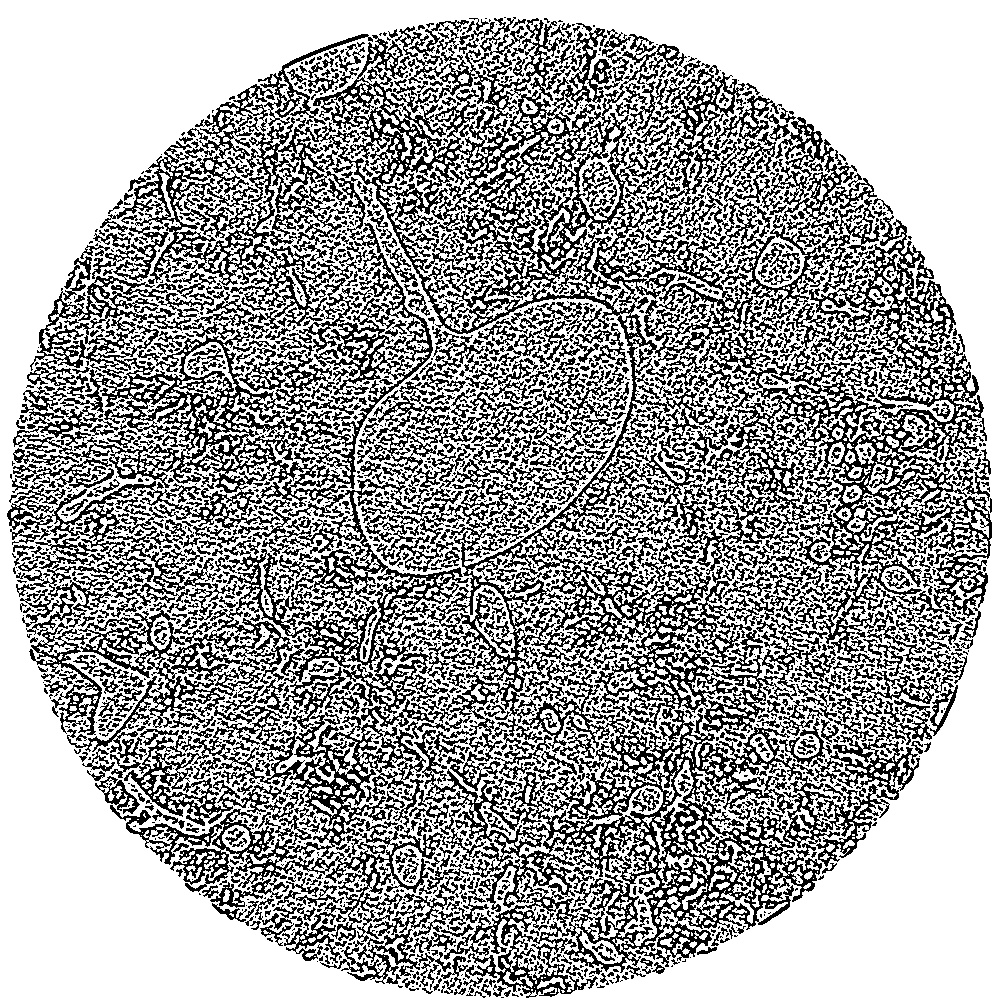
\includegraphics[width=3cm]{thresh/adap1.jpg}\\
     b)
   \end{minipage}
    \begin{minipage}[c]{0.3\textwidth}
	\centering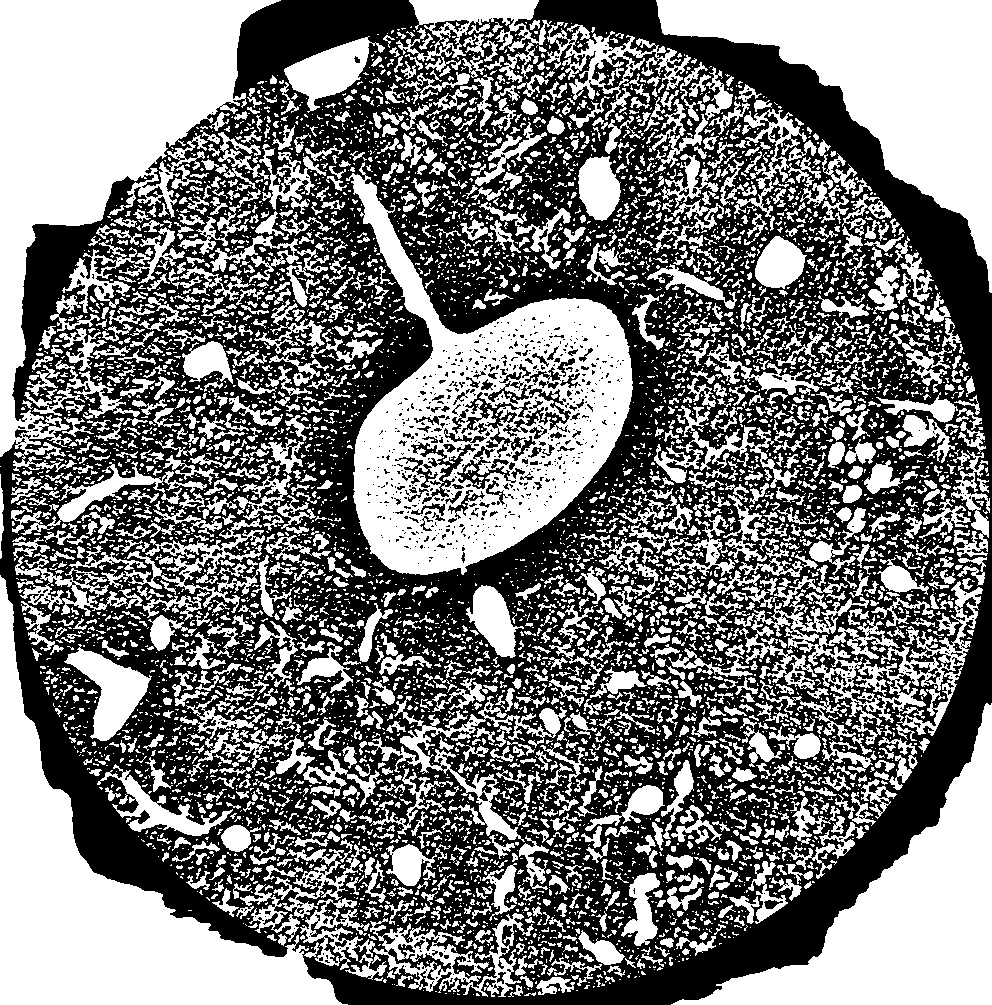
\includegraphics[width=3cm]{thresh/adap2.jpg}\\
     c)
   \end{minipage}
    \begin{minipage}[c]{0.3\textwidth}
	\centering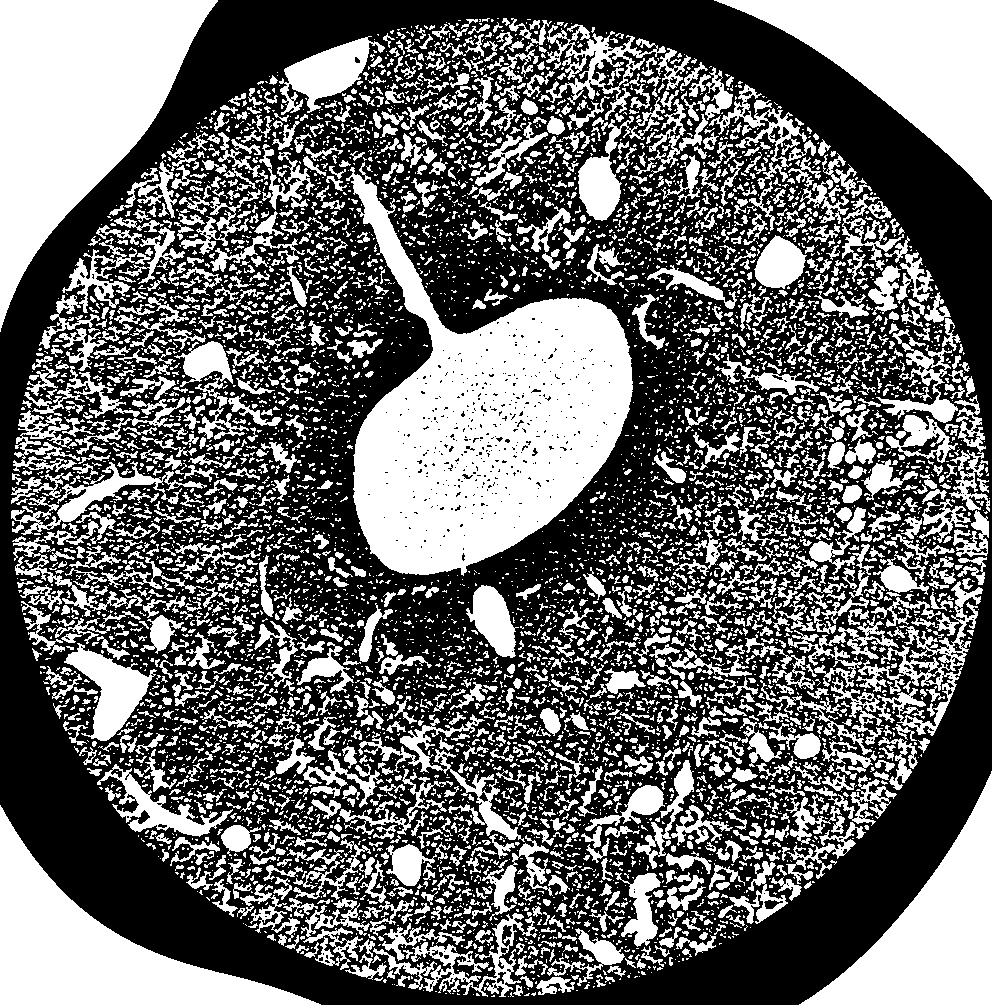
\includegraphics[width=3cm]{thresh/adap3.jpg}\\
     d)
   \end{minipage}
    \begin{minipage}[c]{0.3\textwidth}
	\centering\includegraphics[width=3cm]{thresh/otsu.jpg}\\
     e)
   \end{minipage}
    \begin{minipage}[c]{0.3\textwidth}
	\centering\includegraphics[width=3cm]{thresh/perc.jpg}\\
     f)
   \end{minipage}
    \begin{minipage}[c]{0.3\textwidth}
	\centering\includegraphics[width=3cm]{thresh/perc2.jpg}\\
     g)
   \end{minipage}

	\caption[Prahování]{Prahování - a) původní obraz; b) adaptivní prahování pro okénko 11x11; c) adaptivní prahování pro okénko 121x121; d) adaptivní prahování pro okénko 501x501; e) Otsu prahování; f) Percentní prahování pro 15\%; g) Percentní prahování pro 85\%}
\end{figure}
\subsection{Detekce hran}
Nejprve definujme co to je hrana. V obraze je hrana místem kde dochází k nespojitosti v barvě, jasu případně textuře nebo jiných obrazových parametrů. Hranu. Segmentace s pomocí detekce hran využívá právě této vlastnosti a úvahy, že každý objekt v obraze bude ohraničen hranou.
\subsubsection{Využití znalosti polohy hranic}
Pokud obraz na němž se snažíme hrany detekovat předzpracujeme například prahováním je možné uvažovat jistou aprioprní informaci minimálně o pravděpodobné poloze hrany a také jejímu tvaru. Tyto informace můžeme získat například aplikací segmentace na obraze s nižším rozlišením. Můžeme také využít například polohu významných hranových buněk. Pokud máme tedy nějakou takovou apriorní informaci o pravděpodobné poloze a tvaru hranice může proložit apromační křivkou a tím hranici zpřesnit.
\subsubsection{Postupné dělení spojnic}
Tato metoda pracuje se vstupem který tvoří obraz a koncové body hranice. Zároveň je nezbytné aby obraz, který je zkoumaný neobsahoval příliš mnoho šumu. Dalším předpokladem je tvar hranice. Tuto metodu použijeme pokud nepředpokládáme příliš zakřivenou hranici. Princip této metody je takový že vytvoříme spojnici mezi každými dvěma body na hranici. Uprostřed této spojnice nalezneme normálu a právě na ní hledáme další body ležící na hledané hranici. Z nalezených bodů vezmeme ten, který je nejblíže spojnice mezi již detekovanými body a má nadprahovou hondotu velikosti hrany je považován za nový hraniční bod. Tento proces se opakuje - jedná se tedy o iterační metodu.
\subsubsection{Cannyho hranový detektor}
Tato metoda přepodkládá málo zašumněný obraz, ten je samozřejmě vhodné předzpravat vhodnou filtrací šumu. Někdy se přímo v algoritmu Cannyho hranového detektoru využívá Gaussův filtr (popsaný v kapitole \ref{gauss}). Dalším krokem je výpočet první derivace - gradientu. V tomto případě se často používá Sobelův operátor. Jeho hlavními výhodami je relativně nízká citlivost na šum a také skutečnost, že kromě velikosti gradientu, který reprezentuje hranu, také její směr. Sobelův operátor má pro velikost 3x3 následující tvar:
$$
h_1 = \left[
\begin{matrix}
1&2&1\\
0&0&0\\
-1&-2&-1
\end{matrix}
\right],
h_2 = \left[
\begin{matrix}
-1&0&1\\
-2&0&2\\
-1&0&1
\end{matrix}
\right],
h_3 = \left[
\begin{matrix}
0&1&2\\
-1&0&1\\
-2&-1&0
\end{matrix}
\right], ...
$$
 Následně jsou nalezeny lokální maxima. V praxi se toto provádí metodou Non-maximum supression (popsanou v kapitole \ref{nonMaxSup}). Tento krok zajišťuje, nalezení hrany v místě největšího gradientu. Tento krok je někdy také označen jako \textit{Thinning - ztenčení}.\\
Nyní tedy máme v obraze označeny všechny hrany bez ohledu na jejich vlastnosti a význam. V posledním kroku tohoto algoritmu jsou vybrány pouze významné hrany. Určíme tedy dva prahy $T_1 < T_2$. Pro jednotlivé body $f(x,y)$:
$$
(x,y)
\Bigg\{
\begin{matrix}
f(x,y) \geq T_2 \;& x,y\ je\  hranový\ bod\\
T_1 \leq f(x,y) < T_2&x,y\ je\ hranový\ pokud\ \exists\ sousední\ hranový\ bod\\
T_1 \leq f(x,y) < T_2&x,y\ není\ hranový\ pokud\not\exists sousední\ hranový\ bod\\
f(x,y) < T_1 \; & x,y\ není\ hranový
\end{matrix}
$$
 \begin{figure}[htp!]
  \centering
  
   \begin{minipage}[c]{\textwidth}
	\centering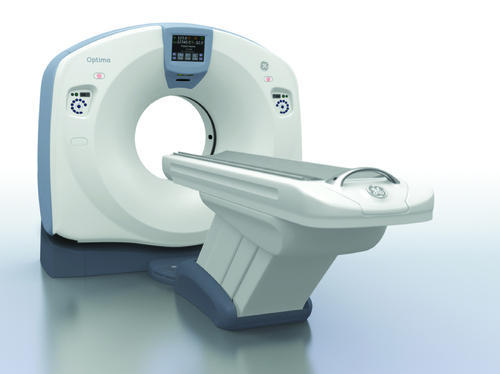
\includegraphics[width=3cm]{ctmach.jpg}\\
     a)
   \end{minipage}
    \begin{minipage}[c]{0.3\textwidth}
	\centering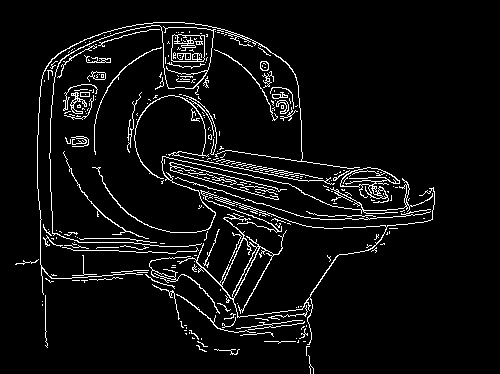
\includegraphics[width=3cm]{canny/Canny10_50.jpg}\\
     b)
   \end{minipage}
    \begin{minipage}[c]{0.3\textwidth}
	\centering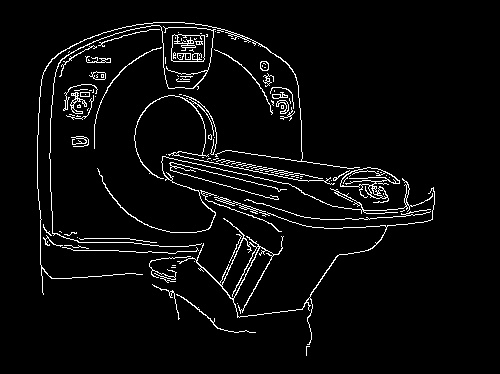
\includegraphics[width=3cm]{canny/Canny20_100.jpg}\\
     c)
   \end{minipage}
    \begin{minipage}[c]{0.3\textwidth}
	\centering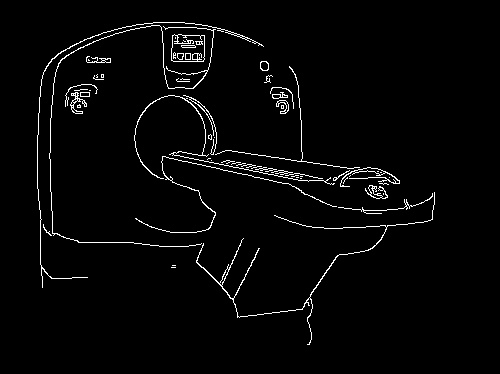
\includegraphics[width=3cm]{canny/Canny100_200.jpg}\\
     d)
   \end{minipage}


	\caption[Cannyho hranový detektor]{Cannyho hranový detektor - a) původní obraz - CT ; b) nastavení prahů na $T_1$ = 10 a $T_2$ = 50; c)  nastavení prahů na $T_1$ = 20 a $T_2$ = 100; d) nastavení prahů na $T_1$ = 100 a $T_2$ = 200}
\end{figure}
\subsubsection{Derivace a konvoluční masky}
V předchozí kapitole bylo popsáno použití Sobelova oprátoru k nalezení hran. Sobelův operátor samozřejmě není jediný, který je možné použít, další konvoluční masky jsou například \textbf{Robertsův operátor} $2x2$:
$$
h_1 = \left[
\begin{matrix}
1&0\\
0&-1
\end{matrix}
\right],
h_2 = \left[
\begin{matrix}
0&1\\
-1&0
\end{matrix}
\right]
$$
Gradient je pak vypočítán následně
\begin{equation}
|g(x,y) - g(x+1,y+1)|+|g(x,y+1)-g(x+1,y)|
\end{equation}
Nevýhodou tohoto operátoru je vysoká citlivost na šum vstupního obrazu. Důvod je zřejmý, vzhledem k tomu, že zkoumané okolí je velmi malé má velký vliv na výpočet každý zkoumaný bod obrazu.\\
Dalším je \textbf{Operátor Prewittové}, kteý  má pro okolí $3x3$ následující tvar:
$$
h_1 = \left[
\begin{matrix}
1&1&1\\
0&0&0\\
-1&-1&-1
\end{matrix}
\right],
h_2 = \left[
\begin{matrix}
0&1&1\\
-1&0&1\\
-1&-1&0\end{matrix}
\right],
h_3 = \left[
\begin{matrix}
-1&0&1\\
-1&0&1\\
-1&0&1
\end{matrix}
\right],...
$$
\textbf{Robinsonův operátor} $3x3$ pak vypadá následně:
$$
h_1 = \left[
\begin{matrix}
1&1&1\\
1&-2&1\\
-1&-1&-1
\end{matrix}
\right],
h_2 = \left[
\begin{matrix}
1&1&1\\
-1&-2&1\\
-1&-1&1\end{matrix}
\right],
h_3 = \left[
\begin{matrix}
-1&1&1\\
-1&-2&1\\
-1&1&1
\end{matrix}
\right],...
$$
Jistě ne posledním ale posledním operátorem, který zmíníme je \textbf{Kirschův operátor} pro okolí $3x3$:
$$
h_1 = \left[
\begin{matrix}
3&3&3\\
3&0&3\\
-5&-5&-5
\end{matrix}
\right],
h_2 = \left[
\begin{matrix}
3&3&3\\
-5&0&3\\
-5&-5&3\end{matrix}
\right],
h_3 = \left[
\begin{matrix}
-5&3&3\\
-5&0&3\\
-5&3&3
\end{matrix}
\right],...
$$
 \begin{figure}[htp!]
  \centering
  
   \begin{minipage}[c]{\textwidth}
	\centering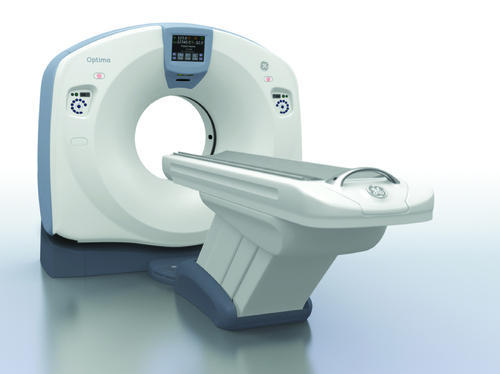
\includegraphics[width=3cm]{ctmach.jpg}\\
     a)
   \end{minipage}
    \begin{minipage}[c]{0.3\textwidth}
	\centering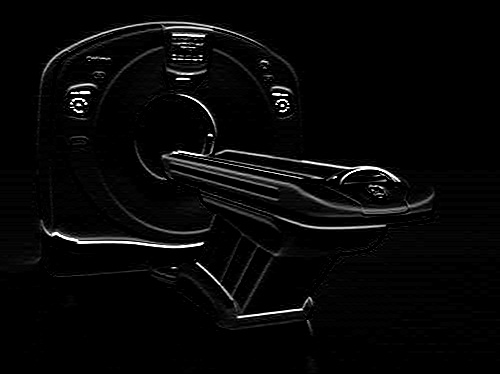
\includegraphics[width=3cm]{convolution/Sobel1.jpg}\\
     b)
   \end{minipage}
    \begin{minipage}[c]{0.3\textwidth}
	\centering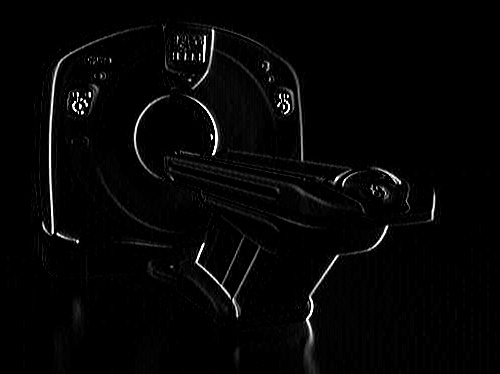
\includegraphics[width=3cm]{convolution/Sobel2.jpg}\\
     c)
   \end{minipage}
    \begin{minipage}[c]{0.3\textwidth}
	\centering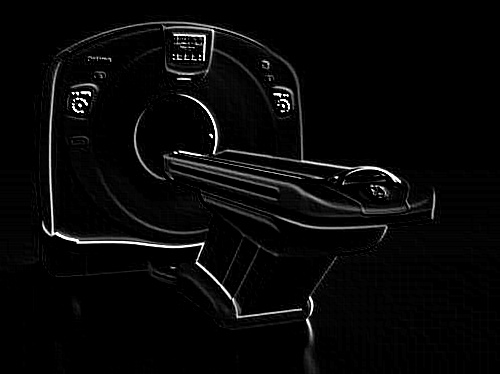
\includegraphics[width=3cm]{convolution/Sobel3.jpg}\\
     d)
   \end{minipage}
    \begin{minipage}[c]{0.3\textwidth}
	\centering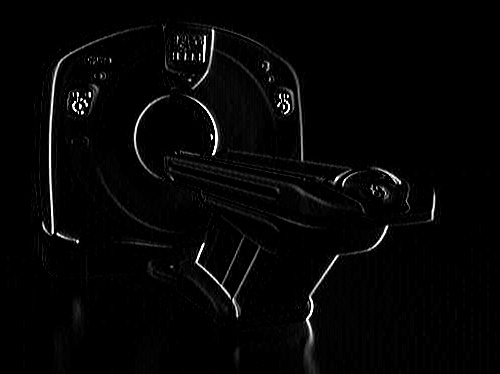
\includegraphics[width=3cm]{convolution/Prewitt1.jpg}\\
     e)
   \end{minipage}
    \begin{minipage}[c]{0.3\textwidth}
	\centering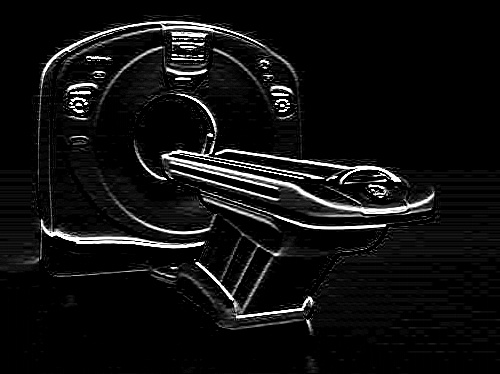
\includegraphics[width=3cm]{convolution/Kirsch1.jpg}\\
     f)
   \end{minipage}
    \begin{minipage}[c]{0.3\textwidth}
	\centering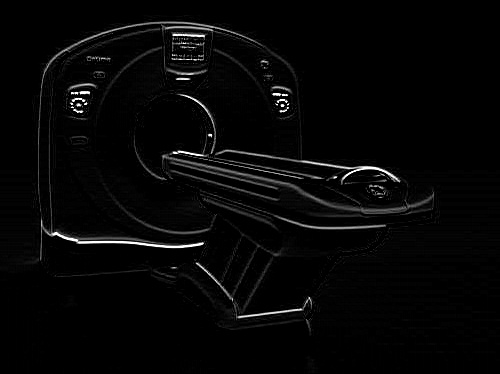
\includegraphics[width=3cm]{convolution/Robinson1.jpg}\\
     g)
   \end{minipage}

	\caption[Konvoluce s různými maskami]{Prahování - a) původní obraz - CT ; b) Sobelův operátor h1; c)  Sobelův operátor h2; d) Sobelův operátor h3; e) Prewitt operátor; f) Kirschův operátor; g) Robinsonův operátor}
\end{figure}\\
Pozn.: Všechny konvoluce se všemi oprátory d) - g) provedeny s $h_1$ maskou popsanou výše.
\subsubsection{Aktivní kontury}
Tato metoda na svém vstupu požaduje mít uzavřenou křivku kolem segmentu, který je nezbytné určit přesně. Je to tedy metoda sloužící především pro zpřesnění výsledků nějaké hrubší segmentace. Hranice je zpřesňována otevřenou nebo uzavřenou spline funkcí (snake)\footnote[14]{Definována D.T. Sandwellem v roce 1987.}. Metoda pracuje na principu minimalizace energie z části určené enregiíí segmentu pod spline funkcí a z druhé části energií křivky získané právě spline funkcí. Tato metoda je vhodná i pro zašumněná data, hlavní nevýhodou je potřeba specifikovat oblast, v níž se segment snažíme nalézt.

\subsubsection{Watershed segmentation}
Do češtiny můžeme přeložit jako \textit{registrace povodím}. Metoda pracuje uvažuje obraz jako krajinu, kde jasové hodnoty v podstatě určují nadmořkou výšku jednotlivých bodu. Do této krajiny je pak vlita imaginární voda. Segmenty se stejou nadmořskou výškou (jasovou hodnotou) jsou pak naplněny vodou a hrany se pak nalézají na hranicích jednotlivých segmentů.
 \begin{figure}[htp!]
  
	\centering\includegraphics[width=5cm]{wattershad.png}\\
	\caption[Watershed segmentation]{Watershed segmentation}
\end{figure}

\subsection{Houghova transformace}
Metoda původně vznikla pro hleání přímek v obraze. Obecně ale s použitím Houghovy transformace (HT) jsme schopni nalézt objekty deného tvaru. HT je vhodná pro zašumněné objekty a použitelná i tehdy je-li v obraze část hledaného objektu zakryta. Nevýhodou je pak fakt, že musíme znát tvar hledaného objektu. Další nevýhodou HT je poměrně malá rychlost a nepřesnosti vzniklé zkreslením objektů.\\
Princip popišmě na jednoduchém hledání přímky v $\mathbb{R}^{2}$ prostoru. Každá přímka v dvojrozměrném prostoru je určena vzdáleností od středu souřadného systému a úhlem, který svírá s jednou s os, řekněme s osou $x$. Tento úhel označme $\sigma$. Každá přímka je tedy dána dvojicí $(r,\sigma)$ neboť rovnice přímky je:
\begin{equation}
x cos(\sigma) + y sin(\sigma) = r
\label{primka}         
\end{equation}
Mějme tedy opět prostor $\mathbb{R}^{2}$ s osami $r$ a $\sigma$. V takovém prostoru se pak každá jedna přímka zobrazí jako jediný bod. Pokud mám tedy v prostoru s osami $x,y$ definován libovolný bod mohu nalézt množinu přímek, které tímto bodem procházejí. Pokud tyto přímky budu postupně dostazovat do rovnice (\ref{primka}) dostaneme v prostoru $r,\sigma$ sinusovku. Pro každý bod $x,y$ pak můžeme vykreslit v prostoru $r,\sigma$ takovou sinusovku. Přímku procházející, všemi těmito body pak nelezneme jako průnik sinusovek v prostoru $r,\sigma$.

 \begin{figure}[htp!]
  
	\centering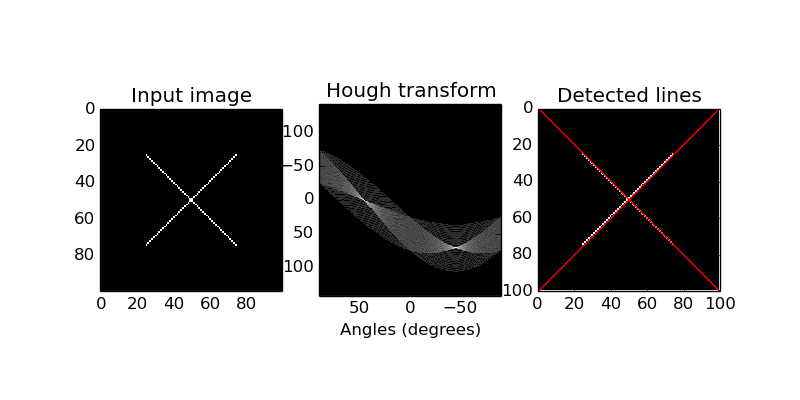
\includegraphics[width=7cm]{hough_trans.png}\\
	\caption[Houghova transformace]{Houghova transformace pro nalezení přímek v 2-D obraze}
\end{figure}
\subsection{Narustání oblastí - Region growing}
Metoda Region growing (RG) pracuje na principu rozdělení obrazu do ploch, které jsou homogenní a to v předem definovaném kritériu nebo vlastnosti. Touto vlastností může být v podstatě cokoliv od hodnoty jasové intenzity pixelu až po sofistikované komplexní popisy. Výhodou je RG je možnost použít na zašumněné oblasti, kde je obtížné hledat hranice. RG pracuje jednoduše na porovnání pixelu se sousedy. Homogenita se určuje následně:
\begin{equation}
\bigg\{
	\begin{tabular}{c|c}
                        $H(R_i) = HOMOGENNÍ$&$ \forall i \in <1,2,..,I$\\ 
		   $H(R_i \cup R_j)\neq HOMOGENNÍ$&$ \forall i,j \in <1,2,..,I\ i\neq j\; 	\land \; R_i\ soused\ R_j$\\ 

	\end{tabular}           
\end{equation}
Přičemž $I$ je počet oblastí $R_i$ a $R_j$ jednotlivé oblasti $H(R_i)$ pak vyjadřuj homogenitu 

\subsection{Náhodné Markovské řetězce}
S Markovskými řetězci se nejšastěji setkáváme při práci s náhodnými procesy ten můžeme za Markovský řetězec označit platí-li: pravděpodobnost přechodu do následujícího stavu závisí pouze na stavu současném (nikoliv na stavech předchozích). V oblasti práce s obrazy tak můžeme použít stejnou myšlenku a to: význam bodu je závislý jen a pouze na významech bodů přímo sousedících. Mějme tedy pixel $x$ a ten je definovaný svým příznakem, respektive příznakovým vektorem $\overrightarrow{f_x}$. Tímto příznakem může být opět obecně cokoliv, nejjednodušší je použití jasu příslušného bodu. Dále mějme množinu všech příznaků, resp. přiznakových vektorů:
\begin{equation}
f = \{\overrightarrow{f_x} : x \in \mathbf{I}\}
\end{equation}
Dále mějme množinu všech označení (labelů) $\mathbf{L} = \{ pozadí, popředí\}$. Každé prvek množiny $\mathbf{L}$ je přiřazen k $x$ a nazýváme jej skrytou proměnnou. Máme-li segmentovaný o rozměrech $AxB$ pak máme $|\mathbf{L}|^{A*B}$ možných výsledků. Tuto hodnotu označme $|\Omega|$. Cílem segmentační úlohy je samozřejmě z množiny všech možných řešení vybrat to správné na základě pravděpodobnostní míry. Hledáme teda $w^*$ maximalizující podmíněnou pravděpodobnost $P(w|f)$. Platí: $w=\{ w_x : x \in \mathbf{L}\}$ a hledáme tedy odhad maximální aposteriorní pravděpodobnosti (MAP):
\begin{equation}
w^{*MAP} = \argmax_{w\in \Omega}P(w|f)
\end{equation}
S využitím Bayesova pravidla můžeme zapsat
\begin{equation}
P(w|f) = \frac{P(f|w)P(w)}{P(f)}
\end{equation}
vzhledem k tomu, že $P(f)$ je konstatní můřeme dělitele předchozí rovnice vynechat. Tímto krokem a dosazením převádíme na úlohu opmalizace minimální energie dat + energie spojitosti. V praxi je náhodné pole často definováno jako graf a následně použita metoda Graph-Cut.

\subsection{Metody založené na zkoumání tvaru}
\subsubsection{Gaborovy filtry a K-means}

\subsubsection{Metoda založená na vlastních číslech Hessovi matice - Frangiho filtr}
Hessova matice je maticí druhých parciálních derivací skalární funkce a má následující tvar:

\begin{equation}
H(f) = \left| \begin{array}{cccc}
\frac{\partial^2 f}{\partial x_{1}^2} & \frac{\partial^2 f}{\partial x_1 \partial x_2} & ... &  \frac{\partial^2 f}{\partial x_1 \partial x_n}\\
\frac{\partial^2 f}{\partial x_2\partial x_1} & \frac{\partial^2 f}{\partial x_2^2} & ... &  \frac{\partial^2 f}{\partial x_2 \partial x_n}\\
... & ... & ... & ...\\
\frac{\partial^2 f}{\partial x_n \partial x_1} & \frac{\partial^2 f}{\partial x_n \partial x_2} & ... &  \frac{\partial^2 f}{\partial x_n^2}
\end{array} \right|
\end{equation}
Frangiho segmentační filtr pracuje s faktem, že cévy jsou válcovité struktury. Pro každý jeden voxel tedy zkoumá okolí a takovéto struktury hledá.\\ V problematice segmentace je možné použít \\\
Hessovu matici použivá jako konvoluční filtr. Následně provedeme dekompozici na vlastní vektory. Vzhledem k tomu, že je použita matice 3x3 dostaneme pro každý voxel obrazu tři vlastní vektory. Tato sada vektorů reprezentuje zkoumaný voxel v novém ortonormálním souřadnicovém systému a obsahuje infomraci o zakřivení zkoumaného obrazu. Vlastní čísla kvantifikují velikost zakřivení v jednotlivých směrem a je tedy možné je použít pro hledání různých typů struktur (viz tabulka XX). Díky tomuz je možné najít cévám podobné obrazy na základě zkoumání vlastních vektorů Hessovy matice.\\
Mějme tedy vlastní čísla $\lambda_1 \leq \lambda_1 \leq \lambda_1$ cévy nebo obecněji válcovité struktury pak v odpovídají myšlence, že ve dvou směrech je zakřivení velké a ve třetím směru naopak malé. tj.:

\begin{equation}
|\lambda_1| \approx 0, |\lambda_1|\ll |\lambda_2|, |\lambda_3|
\end{equation}
Pro usnadnění klasifikace jednotlivých struktur je ve Frangiho filtru definováno několik poměrů například:
 \begin{equation}
R_A = \frac{|\lambda_2|}{|\lambda_3|}
\end{equation}
, který rozlišuje válcovitých od dekovitých struktur. Jak bylo zminěno výše $ \lambda_2$ a $\lambda_3$ jsou v případě cév téměř stejně velké a hodnota $\lambda_1$ je naopak malá po celé délce struktury. Pokud se jedná plochou deskovitou strukturu jesou první dvě hodnoty malé (tj. $\lambda_1$ a $\lambda_2$) a pouze hodnota $\lambda_3$ je výrazně vyšší. Pokud se tedy jedná o válcovitou cévám podobnou strukturu, blíží se poměr $R_A$ hodnotě $1$. Naopak pokud bude hodnota tohoto poměru v blízkosti $0$, jedná se o plochou strukturu.\\
Definujme dále poměr $R_B$: 
 \begin{equation}
R_B = \frac{|\lambda_1|}{\sqrt{|\lambda_2||\lambda_3|}}
\end{equation}
, díky němuž je možné oddělit válcovité a kulovité struktury. Kulovité struktury mají vlastní čísla Hessovi matice zhruba stejně velká. $R_B$ tedy dosahuje svého maxima blížícího se 1 právě pro kulovité struktury, zatímco pro ostatní hodnotu blížící se 0.\\
Další informaci o struktuře a tvaru můžeme získat z tzv. \textit{Frangi's structureness measure} (v češtine možno říci Frangiho míru strukturality):
 \begin{equation}
S = ||H||_F = \sqrt{\sum_{j\leq D}\lambda^2} = \sqrt{\sum \lambda_1^2 + \lambda_2^2 + \lambda_3^2}
\end{equation}
Tato míra je Frobeniovou normou matice a díky ní můžeme oddělit šum a strukturu nebo oblast zájmu. Frobeniova norma uvažuje velikost všech tří vlastních čísel z nichž pro libovolnou strukturu bude minimálně jedno obsahovat vysokou hodnotu narozdíl od šumu. \\
Frangiho celková míra podobnosti cévní struktuře je pak spočítána následujícím způsobem:
 \begin{equation}\label{Frangiho celková míra}
V(x,s) = \Big\{   \begin{array}{c}
0 \;\;\;\;\;\;\;\;\;\;\;\;\;\;\;\;\;\;\;\;\;\;\;\;\;\;\;\;\;\;\;\;\;\;pokud\; \lambda_2 > 0 \;nebo\; \lambda_3 > 0\\
(1-exp(\frac{-R_A^2}{2\alpha^2}))exp(\frac{-R_B^2}{2\beta^2})(1-exp(\frac{-S^2}{2 \gamma^2}))\;\;\;\;\;jinak
\end{array}\end{equation}
Kde $\alpha,\beta$ a $\gamma$ jsou prahové hodnoty definující citlivost Frangiho na jednotlivé typy struktur a šum. Dle definice Frangiho míry  \ref{Frangiho celková míra} jsou také zanedbány voxely, pro něž jsou vlastní čísla matice $\lambda_2$ a $\lambda_3$ větší než 0. Právě tato vlastnost indikuje, že se jedná o voxely s nízkou optickou absorbcí na pozadí. Pro přehlednost je význam jednotlivých vlastních čísel Hessovy matice uveden v následující tabulce:
\begin{center} 
\begin{tabular}{c c c c c}
\hline
$\lambda_1$ & $\lambda_2$  & $\lambda_3$ & Tvar struktury& \\
\hline
malé & velké  & velké & válcovitá &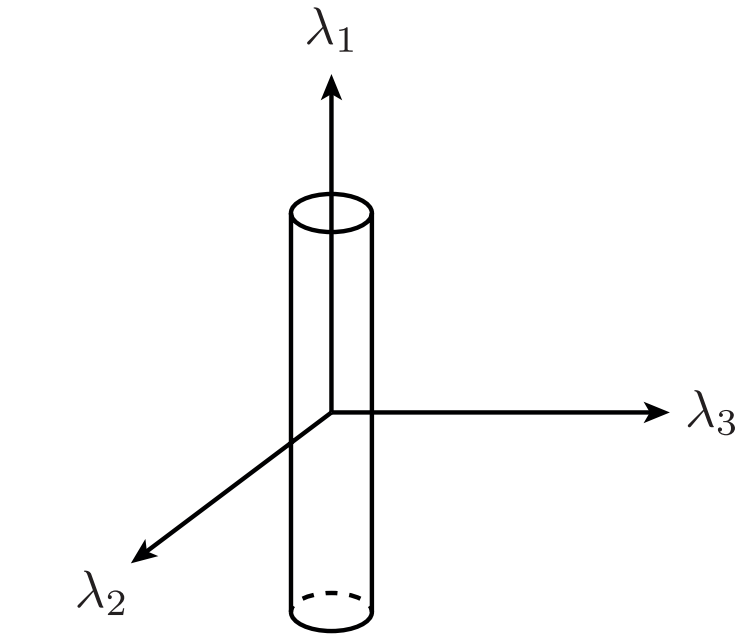
\includegraphics[width=1.0cm]{imgs/tube.png} \\
\hline
malé & malé  & velké & plochá, talířovitá &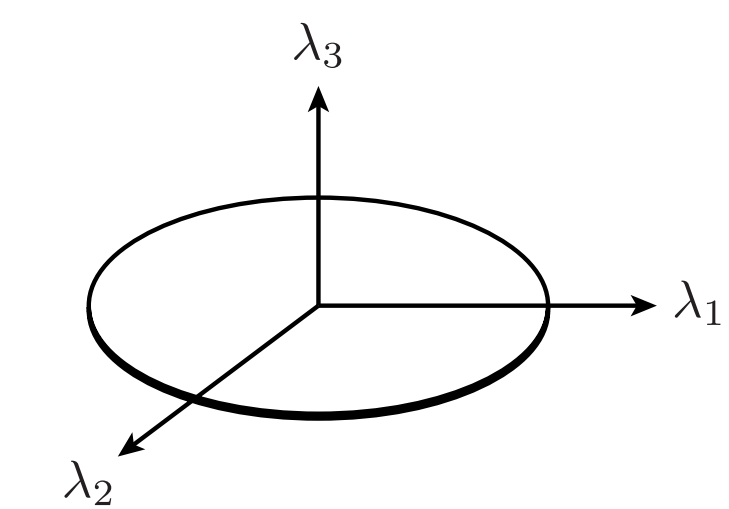
\includegraphics[width=1.0cm]{imgs/plate.png} \\
\hline
velké & velké  & velké & kulovitá &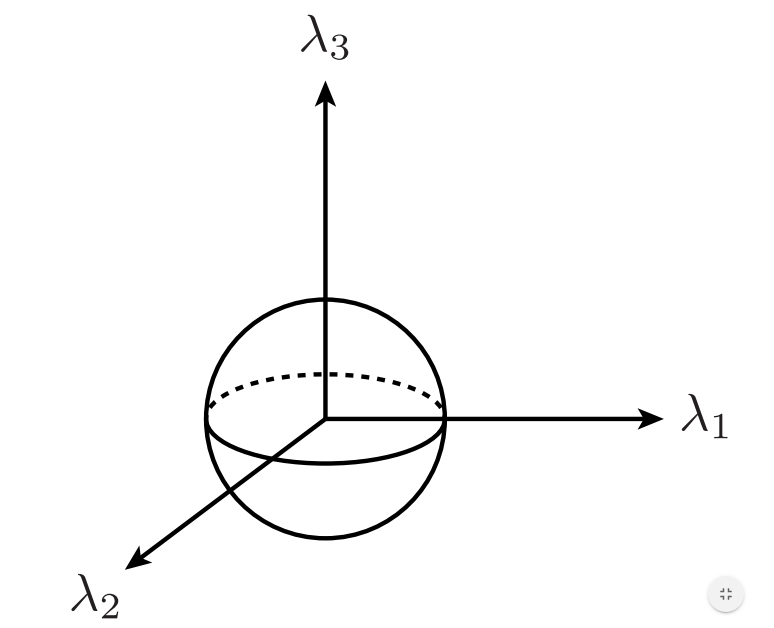
\includegraphics[width=1.0cm]{imgs/blob.png} \\
\end{tabular}
\end{center}
Frangiho filtr je vhodné použít opakovaně v různých měřítkách a různém natočení Hessovy matice v 3D obraze. Výsledky jednotlivých filtrací jsou pak zkombinovány celková míra důvěry ve skutečnost že se jedná o cévu je spočetena dle následujícího vztahu:
 \begin{equation}
\hat{V}(x) = \max_{s_{min}\leq s\leq s_{max}} v(x,s)
\end{equation}
\chapter{Registrace obrazových dat}
Problém fúze obecně $N$ snímků s různým rozlišením a jinou orientací je v podstatě problémem registrace obrazových dat. Zde je cílem prolnout dva snímky do jednoho. Tento cíl je možné přeformulovat jako hledání vhodné transformace, která zajístí že obrazy A a B budou po transformaci jednoho z nich totožné. Tedy bude platit:\\
 $$A = Trans.(B) $$
nebo
$$ Trans.(A) = B$$
Vzhledem k tomu, že v našem případě se budeme pokoušet registrovat dva obrazy přičemž jeden zobrazuje pouze část druhé, představme si \textbf{A} a \textbf{B} jako množiny a pak výše uvedený vztah můžeme definovat následujícím způsobem:
$$A \subset Trans.(B)$$
nebo 
$$B \subset Trans.(A)$$
K získání vhodné tranasformace mohou vést dvě cesty cesta přímá a iterativní. Přímé algoritmy registrace obrazových dat respektive nalezení vhodné transformace pracují na předpokladu, že máme dvojice bodů vzájemně si odpovídajících na každém z obrázků, jejichž fúzi se snažíme provést. V tomto případě je možné nalézt transformaci pomocí řešení soustavy lineárních rovnic a celý proces může fungovat jednokrokově. Pokud ovšem není možné přesně určit výše zmíněnou dvojici bodů na každých dvou obrazech které chceme prolnout je vhodnější iterativní přístup. Ten se v několika krocích snaží transformaci určenou jako počáteční modifikovat, tak aby došlo k co nejlepšímu spojení obrazů. \\
Abychom dokázali určit, co která transformace je "lepší" je třeba najít veličinu, na níž kvalitu prolnutí obrazových dat budeme určovat. Jinými slovy hledáme funkci $\hat{T}$ takové, že platí:
\begin{equation}
 \centering
	\hat{T} = arg \min_{T \in H}\mathbf{K}(I_{1}(x,y,z),\mathbf{g}(I_{2}(\mathbf{T}(x,y,z)))) 
\end{equation}
kde $\mathbf{K}$ je kriteriální funkcí určující míru podobnosti transformovaných obrázů. $\mathbf{T}$ je množina funkcí které pro trojrozměrný obraz zobrazují $\mathbb{R}^{3}\rightarrow\mathbb{R}^{3}$. $,\mathbf{g}$ je $\mathbb{R}\rightarrow\mathbb{R}$ - interpolační funkce. Funkce $\hat{T}$ nechť je potom hledanou tranformační funkcí.\\

\section{Rigid / Non-Rigid body registrace}
Problém registrace obrazových dat je tedy proložení dvou rozdílných vstupních obrazů do jednoho a tím i nalezení vhodné transformace. To je možné několika způsoby dva hlavní směry jsou Rigid body a Non-Rigid body registrace.
\subsection{Rigid body registrace}
Jak název napovídá z překladu anglického \textit{rigid} = \textit{pevný, tuhý, neohebný} jedná se o transformace, které vlastní prostor obrazu nijak nedeformují a zachovájí jeho tvar pevný a němenný. Jinými slovy tento způsob registrace využívá při transformaci pouze lienárních globálních transformací jako je rotace a transalce.\\
Nespornou a hlavní výhodou tohoto přístupu, je nízký počet stupňů volnosti. Například uvažujeme-li prostor $\mathbb{R}^{2}$ můžeze z možných tranformací uvažovat jen translace ve směru $x$ a $y$ a rotaci. S každým dalším rozměrem samozřejmě počet možných transofrmací narůstá. Pro $\mathbb{R}^{3}$ už je translace ve třech směrech $x,y,z$ a rotace kolem těchto tří os. Pro $\mathbb{R}^{3}$ máme tedy šest stupňů volnosti přesto stále neuvažujeme žádnou deformaci obrazu, která by počet možných transofrmací extrémně navýšila. 
 \begin{figure}[htp!]
  \centering
   \begin{minipage}[c]{0.3\textwidth}
     \centering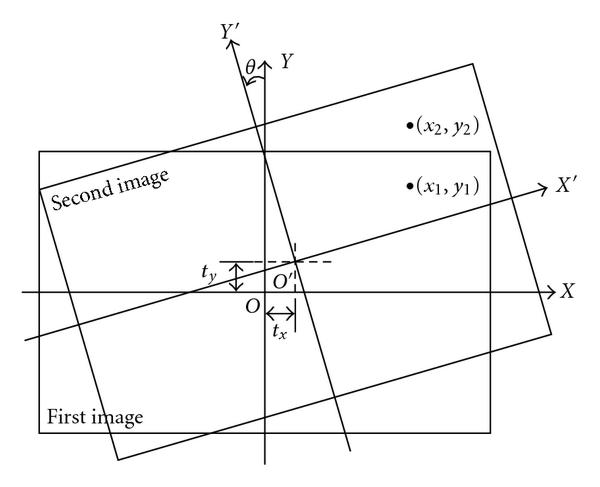
\includegraphics[width=3cm]{Rigid-body-transformation-scale-1.png}\\
     a)
   \end{minipage}
    \begin{minipage}[c]{0.3\textwidth}
     \centering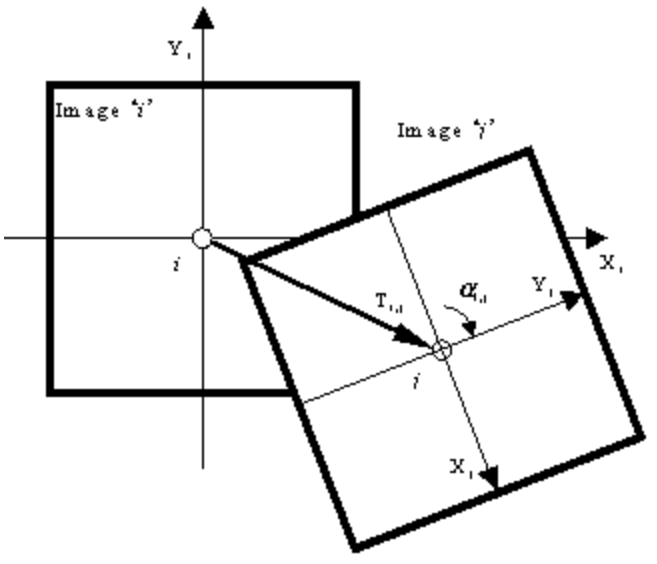
\includegraphics[width=3cm]{rigid2.png}\\
      b)
   \end{minipage}
	\caption[Rigid-body transformace]{Rigid-body transformace}
\end{figure}


\subsection{Non-Rigid body}
Oproti výše zmíněné Rigid body registraci, uvažuje non-rigid body kromě globálních linérních transfromací navíc lokální transformace a také nelineární transformace. Tato skutečnost znamená, že obraz není uvažován jako pevný objekt, ale dochází k jeho deformaci. 
 \begin{figure}[htp!]
  \begin{minipage}[c]{0.5\textwidth}
     \centering\includegraphics[width=3cm]{nonrigid.png}\\
     a)
   \end{minipage}
  \begin{minipage}[c]{0.5\textwidth}
     \centering\includegraphics[width=3cm]{nonrigid2.png}\\
     b)
   \end{minipage}
   
      \caption[Non-Rigid-body transformace]{Non-Rigid-body transformace}
\end{figure}
\newpage
\subsection{Afinní transformace}
Ačkoliv se afinní transformace často řadí mezi Rigid body transformace uvažuje kromě translačních a rotačních pohybů ještě zkosení a také změnu měřítka. Tento typ transformace respektuje rovnoběžnost a také poměr velikostí jednotlivých úsečet.

 \begin{figure}[htp!]
  \centering
   \begin{minipage}[c]{0.3\textwidth}
     \centering\includegraphics[width=5cm]{afinni.png} \\
     a)
   \end{minipage}
   \hspace*{1cm}
    \begin{minipage}[c]{0.3\textwidth}
     \centering\includegraphics[width=3cm]{afinni2.png} \\
     b)
   \end{minipage}

      \caption[Afinní transformace]{Afinní transformace}
\end{figure}

\subsection{Výhody a nevýhody jednotlivých přístupů a jejich souvislost s snímáním pacienta}
Výhoda Rigid body transformace již byla naznačená výše a to je především malý počet stupňů volnosti. To vede k jednoduchému řešení případného problému. V leékařských zobrazovacích metodách se  dá použít v případech, kdy se neočekává změna tvaru zkoumaného objektu. Například dochází-li ke snímkování kostí uspaného pacienta, zde se dá předpokládat, že pokud pacient nezmění polohu, bude se při registraci obrazových dat jednat o Rigid body transformaci. \\
Naopak non-rigid body transformace se dá předpokládat třeba při snímání plic. Předpokládejme, že pacient dýchá a tím pádem i v relativně krátkém časovém okamžiku plíce mění svůj tvar. Stejné to bude například i pro srdce, které bije. Toto platí především u  snímkování pacienta, které trvá delší dobu než je několik vteřin.\\
Rozumným kompromisem se tedy zdá být afinní transformace, která je v oblasti zpracování obrazu pravděpodobně nejvíce využívaným přístupem. Její zápis je podobně jednoduchý jako zápis lineárních transformací Rigid body transformace, ale narozdíl od ní nabízí mnohem širší možnosti díky využití zkosení a změny měřítka.
\section{Metody registrace obrazových dat}
Metod, pro registraci obrazových dat je celá řáda, všechny ovšem mají několik základních kroků, kterými jsou:
\begin{enumerate}
\item Detekce vlastností - tento krok zajišťuje nalezení významných objektů a vlastností registrovaných obrazů jako jsou například hrany, rohy, uzavřené hraniční oblasti.
\item Porovnání vlastností - dále je samozřejmě nutné porovnat významné vlastnosti všech registrovaných obrazových dat a najít nejlepší shodu. Důležité pro tento bod je také stanovit  metriku přes kterou budeme hodnotit shodnost vlastností získaných v kroku 1). Cílem je ideálně ke každému významnému objektu obrazu A najít korespondující vlastnost, bod nebo objekt v obrazu B.
\item Definice transformace - hledáme mapovací funkci, která má za cíl registrovaný obraz co transformovat tak, aby se co nejlépe překrýval s obrazem referenčním. Může se jednat o rotaci, translaci, zkosení, změnu měřítka a mnoho dalších transformací.
\item Vlastní transformace obrazu a převzorkování - v tomto závěrečném kroku je registrovaný obraz transformován aplikací mapovací funkce, interpolován a následně dojde k vlastní proložení obrazů.
\end{enumerate}
 \begin{figure}[htp!]
  
	\centering\includegraphics[width=5cm]{reg_scheme.png}\\
	\caption[Obecné schéma registrace obrazových dat]{Obecné schéma registrace obrazových dat. 1) detekce významných bodů; 2) jejich porovnání a nalezení odpovídajících bodů v registrovaných obrazech; 3) nalezení mapovací funkce; 4) aplikace transformace a proložení}
\end{figure}
\subsection{Bodová registrace}
Bodová registrace využívá přesně určených korespondujících bodů nalezení mapovací funkce. Nezbytné je nalezení odpovídajících si bodů ve všech registrovaných obrazech. Tranformace (mapovací funkce) se pak hledá taková, aby minimalizovala vzdálenost těchto bodů.\\
V praxi je možné bodou registraci realizovat umístěním referenčním značek před zahájením snímání obrazu. Bohužel při snímání CT snímků takové umístění značek možné není. Je tedy nutné významné body najít buď automaticky, jako významné body v obraze je nechat ručně zadat vyšetřujícího lékaře. Nalezení korespondujících bodů ovšem vyžaduje naprostou přesnost při určování souřadnic, což například při ručním zadání může být významným problémem. Mějme tedy dva obrazy $A$ a $B$ a dva body $(x,y) \in A$ a $(j,k)\in B$. Cílem bodové registrace pak bude najít takovou transformaci aby bodová chyba $E_bodová$
\begin{equation}
E_bodová = \sum\limits_{1}^n ||(x_i,y_i)-T(j_i,k_i)||
\end{equation}
byla co nejmenší. Máme-li dva registrované dvojrozměrné obrazy a uvažujeme-li Rigid body registraci postačí nám pro nalezení mapovací funkce vzhledem ke třem stupňům volnosti pouze tři určené korespondující body, obecně ale platí, že čím více korespondujících bodů v obraze nalezneme tím, přesnější registrace bude.\\
Významných bodů které jsou v obrazech detekovány může být navzdory předchozí úvaze příliš velké množství, čímž stoupá časovou náročnost výpočtu. Nutností pro metody bodové registrace je tedy nalezení ``rozumného'' počtu bodů, tak aby byla chyba poku možno co nejmenší na druhou stranu příliš nevzrostla výpočetní náročnost.
\subsection{Registrace ploch}
Další možností jak registrovat obrazová data je porovnávat plochy nebo hranice. V tomto případě není nezbytné určovat jednotlivé body naprosto přesně. Nevýhodou ale mohou být souměrné objekty. Pokud totiž registrovaný snímek je souměrný nalezení mapovací funkce není jednouznačné.
\subsection{Registace na základě podobnosti voxelů}
\subsubsection{Cross-correlation}
Výhodou křížové korelace je její jednoduchá implementace a nezávislá na rozdílné jasové intezitě referenčního a registrovaného obrazu. Často se také používá tzv: Normalized cross correlation (NCC). Může sloužit například jako metrika shodnosti nebo rozdílnosti dvou obrazů. Její hlavní výhodou oproti standartní křížové korelaci je nižsší citlivost na změny amplitudy jasových hodnot pixelů a tím pádem méně závislá na osvětlení obou snímků. Standartní spojitá křížová korelace $\varphi_{xy}$ je pro dvě funkce definována následující rovnicí:
\begin{equation}
\varphi_{xy}(t) = \int_{-\infty}^{\infty}x(\tau-t)y(\tau)d\tau
\end{equation}
Křížovou korelaci je také možné normalizovat a oibecně ji lze použín pro libovolný počet dimezí. Pro jednodimenzionální prostor lze její diskrétní tvar zapsat také následujícím způsobem:
\begin{equation}
r_d = \frac{\sum\limits_i [(x[i]-\overline{x})\cdotp (y[i-d]-\overline{y})]}{\sqrt{\sum\limits_i [(x[i]-\overline{x})^2}\sqrt{ \sum\limits_i (y[i-d]-\overline{y})}}
\end{equation}
Tato rovnice normalizuje výsledky křížovavé korelace na $r_d = \pm 1$. 
Transformace registrovaného obrazu je pak určena dle globálního maxima hodnot získaných křížovou korelací. Typický výsledek s jasným globálním maximem je naznačen na následujícím grafu:

 \begin{figure}[htp!]
  
	\centering\includegraphics[width=5cm]{cc_res.png}\\
	\caption[Výsledek křížové korelace]{Výsledek křížové korelace}
\end{figure}

Křížová korelace zmíněná v předchozím případě má výpočetní náročnost $O(N^2)$. Za účelem zrychlení je možné rychlou Fourrierovu transformaci (FFT). Vycházejme z korelačního teorému, který říká, že vynásobíme-li Fourierovu transformaci jedné funkce\textbf{!!!!!! komplexním konjugátem - complex conjugate } Fourierovy transformace druhé fukce dostaneme Fourierovu transformaci jejich korelace. Tím se z časové oblasti dostaneme do frekvenční oblasti a výsledky dostaneme stejné.\\
Pro zajímavost uvádíme v násleující tabulce porovnání korelace bez a s použitím FFT:
\begin{center}
\begin{tabular}{l|c|c}
 \centering
\bfseries \bfseries Velikost polí & \bfseries Použito FFT & \bfseries Čas výpočtu\\
\hline \hline
512                     &NE& 0.006\\
512                     &ANO& 0.002\\
768                     &NE& 0.013\\
768                     &ANO& 0.003\\
1024                   &NE& 0.025\\
1024                   &ANO& 0.020\\
\end{tabular}
\captionof{table}{Porovnání korelace s a bez použití FFT}
\end{center}

\textit{Using the FFT and the correlation theorem, we accelerate the correlation
computation. The correlation theorem says that multiplying the Fourier transform of
one function by the complex conjugate of the Fourier transform of the other gives the
Fourier transform of their correlation. That is, take both signals into the frequency
domain, form the complex conjugate of one of the signals, multiply, then take the
inverse Fourier transform. This is expressed by: }
\subsubsection{Minimization of variance of intensity ratios}
\textit{Pozn.: Nutno přeložit do češtiny}
Tato metoda je použitelná pouze pro monomodální obrazovou registraci. Vychází z předpokladu, že hodnota každého pixelu (voxelu) může být porovnána z odpovídajícím pixelem druhého obrazu na základě jediného faktoru. Algoritmus je pak tvořen třemi jednoduchými kroky V prvním kroce jsou hodnoty $R(i)$ spočteny jako poměr hodnoty referenčního pixelu (voxelu) $I_R(i)$ a zkoumaného pixelu (voxelu) $I_S(i)$. Tedy
\begin{equation}
 R(i)= I_R(i)/T(I_S(i))
\end{equation}
Druhý krok je potom výpočtem standartní odchylky
\begin{equation}
\sigma_R = 1/N\sum\limits_ {i}(R(i)- \bigtriangleup R(i))
\end{equation}
 kde $N$ je počet pixelů. Ve třetím kroku algoritmu je provedena registrace na zíkladě minimalizace normalizované odchylky 
\begin{equation}
 \sigma_{norm} = \frac{\sigma_R}{\bigtriangleup R}
\end{equation}

\begin{enumerate}
\item Cross-correlation 
\item Fourier domain based cross-correlation, and phase-only correlation
\item Minimization of variance of intensity ratios
\item Minimization of variance of grey values within segments
\item Minimization of the histogram entropy of difference images
\item Histogram clustering and minimization of histogram dispersion
\item Maximization of mutual information (relative entropy) of the histogram
\item Cepstral echo filtering
\item Determination of the optic flow field
\item Minimization of the absolute or squared intensity differences
\item Matching local low-order Taylor expansions determined by the image grey values
\item Implicitly using surface registration by interpreting a 3D image as an instance of a surface in 4D space
\end{enumerate}

\subsection{Registrace na základě informace}
Registraci obrazových dat je možné také provádět na základě množství sdílené informace. Předpokládejme tedy opět dva obrazy poku jeden z nich je možné přímo umístit do obrazu jiného ponese pak celkový registrovaný obraz přesně tolik informace jako první z obrazů. Budou-li se registrované obrazy překrývat částečně pak překrývaná část bude sdílená infomrace a celkovou informaci pak bude možné zapsat následujícím způsobem $A+SDÍLENÁ+B$ ($A$ i $B$ rozumnějmě informace obou obrazů bez sdílené informace). Úkol registrace je tedy možné pojmout jako úlohu maximalizace informace sdílené nebo naopak jako minimalizaci informace celkové.
\subsubsection{Entropie}
Entropie je jmíra neurčitosti určitého jevu. Pokud pracujeme s inforamací, je tuto veličinu klíčové zavézt definována byla Josiah Willard Gibbs jakožto:
\begin{equation}
 S = - k\sum\limits_{i} P_i ln P_i
\end{equation}
kde S je počítaná entropie, $P_i$ pravdědobnost, že nastane stav $i$. Podle Gibbse, který entropii definoval pro termodinamické stavy je $k$ Boltzmannova konstanta $1,380 66×10^{-23} J K^{-1}$.Jednotka entropie je pak stejná jako jednotka tepelné kapacity. My ovšem zaveďme $k = 1/ln(2)$ což platí pro entropii v bitech a odtud dostáváme obecně používaný tvar entropie a to:
\begin{equation}
 S = \sum\limits_{i} P_i log_2 P_i
\end{equation}
Entropie je maximální, pokud je pravděpodobnost všech jevů stejná. Minima dosáhneme pokud množina všech jevů obsahuje jev jistý tedy jev s pravděpodobností rovno jedné. Tím je snadné dopočítat se, že entropie je nulová. V případě informačního přístupu k registraci obrazu je nutné si také uvědomit, že celková entropie se mění pokud budou obrazy vůči sobě pootočené a pokud tedy dojde k interpolaci.  
\subsubsection{Minimalizace celková informace}
Jak již bylo zmíněno výše je registraci obrazových dat možná brát jako úlohu maximalizaci sdílené informace nebo naopak minimalizaci informace celkové. Věnujme se nyní druhému případu, tedy minimalizaci celkové informace. Mějme tedy opět dva intenzitní obrazy $A, B$ a transformace $T(B)$ aplikovanou na druhý z obrazů. Tyto obrazy tedy proložíme jeden druhýma spočtěme pravděpodobnosti $p_{i,j}=p(A(x_k)= i \cap T(B(x_k))$. $X_k$ jsou souřadnice právě zkoumaného pixelu a $i,j$ jsou hodnoty intenzity zkoumaných pixelu trasnformovaného obrazu $B$ a netranformovaného obrazu $A$. Společná entropie je tedy:
\begin{equation}
 S(A,T(B)) = \sum\limits_{i}\sum\limits_{j} p_{i,j}\cdot log_2 (p_{i,j}(A,T(B))
\end{equation}
Pokud jsou obrazy zcela totožné bude platit že celková infomace je rovna informaci jednoho z obrazů. Naopak neponesou-li oba obrazy žádnou společnou infomraci jejich celková entropie bude součtem $S(A,T(B)) = S(A) + S(T(B))$. Z čehož plyne že pro obecné dva obrazy platí:
\begin{equation}
 S(A,T(B)) \leq S(A) + S(T(B)) 
\end{equation}
Jak již bylo zmíněno v úvody této kapitoly dochází-li při tranformaci k rotaci a následné interpolaci dstáváme $S(T(B)) > S(B)$. To může být problém, ptorože celkoá informace a potažmo i entropie roste, i přesto, že obraz je správně umístěn.
\subsubsection{Společná informace}
V angličtině se setkává s pojmem \textit{mutual infomartion} (MI), který je často využíván i v české literatuřě, dále tedy budeme využívat anglickou variantu názvu této metriky pro registraci obrazových dat. MI je druhým možným přístupem k registraci pomocí informace a odstraňuje také prohlém popsaný v výše, tedy fakt že při interpolaci po provedení rotace registrovaného obrazu dojde k navyšení celkové informace ačkoliv by (pokud je obraz správně umisťován) měla celková informace klesat. Myšlenka MI je měřit rozdíl mezi součtem informací jednotlivých obrazů a obrazu celkového (vzniklého výsledkem registrace). Platí tedy:
\begin{equation}
S^{MI}(A, T(B)) = S(A) + S(T(B)) - S(A,T(B))
\end{equation}
po dosazení dostáváme:
\begin{equation}
S^{MI}(A, T(B)) = \sum\limits_i \sum\limits_j p_{i,j} (A,T(B))\cdot log_2 \frac{p_{i,j} (A,T(B))}{p_i(A)p_j(T(B))}
\end{equation}
Tento vzorec je ovšem spolehlivý pouze poku celková informace $S(A,T(B))$ rozse nepatrně. Pokud ovšem máme zašumněný obraz, který má navíc nizkou intenzitu pixelů, může dojít k zkreslení výsledků.\\Za účelem odstranění této skutečnosti můžeme zavést normalizavou MI.
\begin{equation}
S_{NORM}^{MI}(A, T(B)) =\frac{S(A)+S(T(B))}{S (A,T(B))}
\end{equation}
V tomto případě je MI poměrem součtu informací obou obrazů a celkové informace. Vzhledem k tomu, že tento přístup vyjadřuje informaci jak moc je jeden obrázek obsažen v druhém, při registraci se budeme snažit o maxilazaci MI.

\subsection{B-Spline registrace}

\begin{equation}
v(x)=\sum_i p_i \beta_i(x)
\end{equation}

\begin{equation}
\Sigma = \{(x,y,z)|0 \leq x \leq X, 0 \leq y \leq Y, 0 \leq z \leq Z \}
\end{equation}
Nyní definujme síť kontrolních bodů $\Psi$ s rozměry $n_x x n_y x n_z$. Pro body $\Psi_{i,j,k}$ můžeme zapsat:
\begin{equation}
T_{nonrigid}(x,y,z)= \sum_{i=0}^3\sum_{m=0}^3\sum_{n=0}^3 B_i(u)B_m(v)B_n(w) \Psi_{l, m, n} 
\end{equation}
kde $B_x, x\in(i,j,k)$ jsou bázové funkce a $\Psi$ reprezentuje deformační mřížku. Pro registaci obrazových dat v lékařství se nejčastěji používá jako řídící oblast osmiokolí bodu. Vzdálenosti je pak definována následovně:
\begin{equation}
\Omega_x = [\frac{x}{N_x}]-1,\\
\Omega_y = [\frac{y}{N_y}]-1,\\
\Omega_z = [\frac{z}{N_z}]-1
\end{equation}
kde $N$ je počet voxelů pro osy $x,y$ a $z$. Posun každého voxelu v okolí $\Omega(x,y,z)$ je ovlivněn zhruba 64 kontrolními body. Souřadnice 64 kontrolních bodů $CP(l,m,n)$ vypočteme následujicím způsobem:
\begin{equation}
CP_l = [\frac{x}{N_x}-1+i],\\
CP_m = [\frac{y}{N_y}-1+j],\\
CP_n = [\frac{z}{N_z}-1+k]
\end{equation}
Jednotlivé lokální souřadnice $Local(u,v,w)$ v oblasti $\Omega(x,y,z)$ a hodnota je normalizována do intervalu $[0,1]$. Poté je možné zapsat
\begin{equation}
Local_u =\frac{x}{N_x}-[\frac{x}{N_x}],\\
Local_v =\frac{y}{N_y}-[\frac{y}{N_y}],\\
Local_w =\frac{z}{N_z}-[\frac{z}{N_z}]
\end{equation}

\subsection{Non-image based registration}
V českém překladu \textit(neobrazová registrace) zůstaňme ovšem raději u anglického označení. Tato metoda ovšem vyžaduje aby byly obrazy snímány téměř ve stejný čas na stejném místě. Pokud uvažujeme tento požadavek v medicínském prostředí pak to vyžaduje naprostou nehybnost pacienta využití je například v kombinaci CT nebo MRI a ultrazvukového snímání. Myšlenka je taková, že jsou kalibrovány souřadné systémy obou snímků a není třeba k vlastní registraci využívat přímo obrazových dat. Tato technika se v praxi používá například pro záznam polohy chirurgických nástrojů uživáných operačním robotem na jeho rameno. Tyto specifické požadavky definují úzkou oblast použití této metody. 
\section{Optimalizátor}
Důležitým faktorem pro registraci obrazových dat je volba vhodného optimalizátoru. Tím může být například


\begin{enumerate}
	\item Exhaustive - tento optimalizátor vychází z tzv. exhaustive search (exhaustivního vyhledávání) v diskrétní mřížce definované v parametrickém prostoru. Typickým využitím je vykreslení metriky prostoru k získání informace o tom, kolik šumu obsahuje.
	\item Powell - tento optimizátor využívá Brent line search algoritmus. Brentova metoda kombinuje bisekční metodu, secantovou metodu a inverzní kvadratickou interpolaci. Algoritmus se snaží použít potenciálně rychle konvergující secantovou metodu nebo inverzní kvadratickou interpolaci, pokud je to možné, ale v případě potřeby se vrátí zpět k robustnější bisekční metodě.\footnote[15]{Metodu představil australský matematik Richard Pierce Brand \gtrsymBorn~20. dubna 1946 a staví na algoritmu holandského matematika Theodoruse Jozefa Dekkera  \gtrsymBorn~1. března 1927}.
	\item Gradient descent - aktuální pozice se vypočítává následujícím způsobem: $p_{n+1}=o_n+LearningRate\frac{\partial f(p_n)}{\partial p_n}$,  kde $LearningRate$ je hlavním parametrem tohoto optimizátoru.
	\item L-BFGS-B (Limited memory Broyden, Fletcher, Goldfarb, Shannon, Bound Constrained) - tento algoritmus minimalizuje nelineární diferencovatelnou funkci $f(x)$ kde  x je vektor n reálných proměnných. Patří mezi tzv. \textit{quazi-Newtonovské metody} a hlavní výhody přináší při aplikacích s omezenou výpočetní pamětí. Metoda L-BFGS-B využívá odhad inverzní Hessianovy matice k vyhledání nové hodnoty proměnné v prostoru.
\end{enumerate}







\section{Interpolace}
Při transformaci obrazu dochází často k následujícímu problému: Mějme obraz $\mathbf{A}$ a celočíselný souřadnicový systém. Na zmíněný obraz použijeme transoformaci s použitím rotace, translace a dalších možných změn. Jelikož tato transformace je obecná mohou a často také vznikají reálné souřadnice. Pro rekonstrukci obrazu je ovšem nezbytné zobrazit výsledek v celočíselném souřadném systému. Právě za tímto účelem slouží interpolace výsledku, která s využitím hodnot jednotlivých pixelů v 2D obrazu voxelů v 3D obraze a celočíselnou mřížku k výpočtu nových hodnot jednotlivých pixelů/voxelů.
 \subsection{Metoda nejblžšího souseda}
Jinak se tato metad také nazývá "interpolace 0-tého řádu". Její nejvetší devízou je především rychlost. Princip je velmi jednoduchý - zkoumaný pixel získává hodnotu svého nejbližšího souseda. V praxi se často používá varianta zaokrouhlování souřadnic. Hlavními nevýhodami je samozřejmě nepřesnost ovšem na druhou stranu je použitelná pro všechny typy obrazů, jak již bylo zmíněno je velmi rychlá a je jí možné použít pro indexované a černobílé obrazy. Matematicky jí můžeme pro 2D obraz zapsat takto:
\begin{equation}
f(x,y) = \left\{
	\begin{tabular}{c}
                        $p(i,j)\: pro\: i - \frac{1}{2} < x \leq i+ \frac{1}{2},  j - \frac{1}{2} < y \leq j+ \frac{1}{2}$ \\
		   $p(i,j+1)\: pro\: i - \frac{1}{2} < x \leq i+ \frac{1}{2},  j - \frac{1}{2} < y \leq j+ \frac{3}{2}$\\
		   $p(i+1,j)\: pro\: i - \frac{1}{2} < x \leq i+ \frac{3}{2},  j - \frac{1}{2} < y \leq j+ \frac{1}{2}$\\ 
		   $p(i+1,j+1)\: pro\: i - \frac{1}{2} < x \leq i+ \frac{3}{2},  j - \frac{1}{2} < y \leq j+ \frac{3}{2}$
	\end{tabular}           
    \right\}
\end{equation}
kde $(i,j)$ jsou body v prostoru s celočíselnými souřadnicemi, $p(i,j)$ hodnota pixelu na příslušných souřadnicích $(x,y)\in \mathbb{R}^2$.
 \subsection{Bilineární interpolace}
Tato interpolace využívá nikoliv jednoho, jako předchozí metoda, ale čtyři nejbližší pixely z nich počítá vážený průměr. Interpolovanému pixelu, je pak přiřazena hodnota právě váženého průměru. 
\begin{equation}
\begin{split}
f(x,y) = (y-j) [(i+1-x)p(i,j+1)+(x-i)p(i+1,j+1)]+\\
+(j+1-y)[(i+1-x)p(i,jú+(x-i)p(i+1,j)]
\end{split}
\end{equation}
Princip bilineární interpolace je znázorněn i na následujících schématech:
\begin{figure}[ht!]
 \centering
	\includegraphics[width=3cm]{bil_int.png}
	\includegraphics[width=3cm]{bil_intII.png}
	\includegraphics[width=3cm]{bilinear_interpolationIV.png}
	
	\caption[Bilineární interpolace]{Bilineární interpolace}
\end{figure}
 \subsection{Bikubická interpolace}
 Bikubická interpolace je dalším rozšířením na  dvourozměrnou pravidelnou mřížku. K jejímu výpoču se využívá například Langrangeových polynomů, kubického splinu nebo kubické konvoluce.
 \begin{equation}
f(x,y) = \sum\limits_{i,j=0}^3 c_{i}(x)c_{j}(y)f_{ij}
\end{equation}
Kde $c_{i}(x)$ a $c_{j}(y)$  jsou kubické polynomy a $f_{ij}$ hodnota na jednotlivých pozicích tak jak je naznaženo na levém schématu z následujících dvou, které ukazují princip Bikubické interpolace.
 \begin{figure}[ht!]
  \centering
	\includegraphics[width=5cm]{bikubicka2.png}
	\includegraphics[width=5cm]{bikubicka.png}
	\caption[Bikubická interpolace]{Bikubická interpolace}
\end{figure}
 \subsection{Spline interpolace}
 Interpolační spline spočívá v tom, že kromě průchodu všmi uzlovými body $f(x,y)$ má také spojitou alespoň první derivaci. Pro jednorozměrný prostor poté pro $\forall (x_{i})$ platí:
\begin{equation}
\lim_{x\rightarrow x_{i-}}  f'(x) = \lim_{x\rightarrow x_{i+}} f'(x)
\end{equation}

\chapter{Vlastní řešení}
\section{Registrace}
Pro registraci obrazových snímků s různou modalitou byly použity metod
\section{Segmentace}


\begin{enumerate}
\item Vzít microCT snímky
\item Najít a indentifikovat cévy 
\item vybrat N nejlepších snímků = největší informace = největší počet cév větších než D
\item uložit je do vektoru s informacemi o jednotlivých objektech
\item všechny CT snímky a najít cévy
\item najít cévy
\item Projít CT snímky najít njelepší shodu a transformaci
\item použít transormaci na mikroCT a provést registraci
\end{enumerate}

\section{Předpoklady}
\begin{enumerate}
\item RYCHLOST!
\item Přesnost
\item Robustnost
\item Nízká chybovost
\end{enumerate}
\section{Výběr dat }
\section{Transformace obrazu}


\chapter{Závěr}

\newpage
\listoffigures
\listoftables

\begin{thebibliography}{DUSO}
  \bibitem[1]{hugo} Jan Hugo:
    \emph{Velký lékařský slovník}. Maxdorf, Praha, 2015. ISBN: 978-80-7345-456-2 
  \bibitem[0]{medbio} Jozef ROSINA, Leoš NAVRÁTIL:
    \emph{Medicínská biofyzika}. Grada, Praha, 2005. ISBN: ISBN 80-247-1152-4
 \bibitem[0]{lekbio} Vojtěch MORNSTEIN, Ivo HRAZDIRA:
    \emph{Lékařská biofyzika a přístrojová technika}. Neptun, Brno, 2001. ISBN: 80-902896-1-4.
 \bibitem[0]{bak1} Renáta Chylíková:
    \emph{Výpočetní tomografie s vysokým rozlišením – jeho úloha a postavení v radiodiagnostice - Bakalářská práce}. Zdravotně sociální fakulta, Jihočeská univerzita v Českých Budějovicích, 2011.
 \bibitem[0]{bak1} Ing. Michal Španěl,Ing. Vítězslav Beran:
    \emph{Obrazové segmentační techniky}.FAKULTA INFORMAČNÍCH TECHNOLOGIÍ,VYSOKÉ UČENÍ TECHNICKÉ V BRNĚ, 2005
 \bibitem[0]{bak1} Barbara Zitová, Jan Flusser:
    \emph{Image registration methods: a survey}.Department of Image Processing, Institute of Information Theory and Automation, Academy of Sciences of the Czech Republic,2003
\bibitem[SlideShare]{aaa}J. B. Antoine Maintz, Max A. Viergever:
    \emph{An Overview of Medical Image Registration Methods}.Imaging Science Department, Imaging Center Utrecht\\
\bibitem[x]{aaa}Y. Raghavender Rao, Nikhil Prathapani, E.Nagabhooshanam
    \emph{APPLICATION OF NORMALIZED CROSS CORRELATION TO IMAGE REGISTRATION}.  International Journal of Research in Engineering and Technology, eISSN: 2319-1163 | pISSN: 2321-7308.
\bibitem[x]{aaa}Douglas Lyon
    \emph{The Discrete Fourier Transform}. JOURNAL OF OBJECT TECHNOLOGY, ETH Zurich,2010


   \bibitem[WikiSkripta]{WikiSkripta} WikiSkripta:
    \emph{Výpočetní tomografie a Hounsfieldovy jednotky}. \\
    \verb|https://www.wikiskripta.eu/w/V\%C3\%BDpo\%C4\%8Detn\%C3\%AD_tomografie_a_Hounsfieldovy_jednotky|
 \bibitem[Wikipedie]{Wikipedie} Wikipedie:
    \emph{Výpočetní tomografie}. \\
    \verb|https://cs.wikipedia.org/wiki/V\%C3\%BDpo\%C4\%8Detn\%C3\%AD_tomografie|
 \bibitem[what-when-how]{what-when-how} what-when-how In Depth Tutorials and Information:
    \emph{Gray-Scale Image Visualization}. \\
    \verb|http://what-when-how.com/biomedical-image-analysis/gray-scale-image-visualization-biomedical-image-analysis/|
\bibitem[SlideShare]{SlideShare}Archana Koshy:
    \emph{Automatic mosaicing with error equalisation of non-destructive testing images for aerospace industry inspection}.\\
    \verb|https://www.slideshare.net/ArchanaKoshy/ct-physics-ii|

    
\bibitem[Fig 5.1 a)]{RG1}
    \emph{Rigid-body transformation}.\\
    \verb|https://www.researchgate.net/figure/Rigid-body-transformation-scale-1_fig4_43808029|
\bibitem[Fig 5.1 b)]{Rigid-body} Bogdan J. Matuszewski , Lik-Kwan Shark , Martin R. Varley
    \emph{Rigid-body transformation}. Department of Engineering and Product Design, University of Central Lancashire Preston, PR1 2HE, United Kingdom\\
    \verb|https://www.researchgate.net/figure/Rigid-body-transformation-scale-1_fig4_43808029|
\bibitem[Fig 5.2 a)]{Non-rigid body}W R CRUM, DPhil, T HARTKENS, PhD and D L G HILL, PhD
    \emph{Non-rigid image registration: theory and practice}. Division of Imaging Sciences, The Guy’s, King’s and St. Thomas’ School of Medicine, London SE1 9RT, UK\\
\bibitem[Fig 5.2 b)]{Non-rigid body}Sarah McGee
    \emph{Geometric Objects and Transformation}.\\
    \verb|https://slideplayer.com/slide/8241565/|
\bibitem[Fig 5.3 a)]{AfinnTrans}Jaromír FAJT
    \emph{GEOMETRICKÉ TRANSFORMACE V GIS}.Fakulta aplikovaných věd, ZČU Plzeň KMA, obor Gem \\
\bibitem[Fig 5.3 b)]{AfinnTrans}Jaromír FAJT
    \emph{GEOMETRICKÉ TRANSFORMACE V GIS}.Fakulta aplikovaných věd, ZČU Plzeň KMA, obor Gem \\
    \verb|https://cs.wikipedia.org/wiki/Afinn\%C3\%AD_zobrazen\%C3\%AD\#/media/File:Geom_zobrazeni_afinni.svg|
\bibitem[Fig b)]{HistEq2}
    \emph{Histogram Equalization} \\
    \verb|https://www.math.uci.edu/icamp/courses/math77c/demos/hist_eq.pdf|
\bibitem[Fig a)]{HistEq2}Ing. Marek Hrůz Ph.D.
    \emph{ZCU/KKY/MPV} Přednášky z předmětu\\
\bibitem[Fig b)]{HistEq2}Václav Hlaváč
    \emph{Předzpracování obrazů v prostoru obrazů,operace v lokálním sousedství}.České vysoké učení technické v Praze \\
    \verb|http://people.ciirc.cvut.cz/~hlavac/TeachPresCz/11DigZprObr/21ImagPreprocCz.pdf|
\bibitem[Fig b)]{Konvoluce}
    \emph{Diskrétní konvoluce}.České vysoké učení technické v Praze \\
    \verb|http://midas.uamt.feec.vutbr.cz/ZVS/Exercise06/content_cz.php|
\bibitem[Fig b)]{Konvoluce}M ' Barek Nasri, Ahmad El allaoui
    \emph{ Medical Image Segmentation by MarkerControlled Watershed and Mathematical Morphology} \\
    \verb|https://www.researchgate.net/figure/Modelling-of-contours-by-watershed-transform_fig1_266419041|    



\end{thebibliography}
  
%
\end{document}